\documentclass[11pt,american,american]{article}
\usepackage[a4paper]{geometry}
\geometry{verbose,tmargin=2cm,bmargin=2cm,lmargin=2cm,rmargin=2cm,headheight=0.8cm,headsep=1cm,footskip=0.5cm}
\setcounter{secnumdepth}{3}
\usepackage{url}
\usepackage{amsmath}
\usepackage{amsthm}
\usepackage{amssymb}
\usepackage{graphicx}
\usepackage{setspace}
\usepackage{enumerate} %roman enumiration
\usepackage{threeparttable}
\usepackage{algorithmic}
\usepackage{algorithm}
\usepackage{subfigure}
\usepackage[width=.75\textwidth]{caption}
\usepackage{array}
\usepackage[utf8]{inputenc} % Required for inputting international characters
\usepackage[T1]{fontenc} % Output font encoding for international characters
\usepackage{mathpazo} % Palatino font
\usepackage{multirow}
\usepackage{chngcntr}

\counterwithin{figure}{section}
\counterwithin{table}{section}

\pagenumbering{arabic}

\makeatletter
%%%%%%%%%%%%%%%%%%%%%%%%%%%%%% Algorithms
% Define a \HEADER{Title} ... \ENDHEADER block
\newcommand{\HEADER}[1]{\ALC@it\underline{\textsc{#1}}\begin{ALC@g}}
	\newcommand{\ENDHEADER}{\end{ALC@g}}
\renewcommand*{\ALG@name}{Algoritmus}
\algsetup{indent=2em} 
\renewcommand{\algorithmiccomment}[1]{\hspace{2em}// #1} 
\makeatother

%% Use Times New Roman font for text and Belleek font for math
%% Please make sure that the 'esint' package is turned off in the
%% 'Math options' page.
\usepackage[varg]{txfonts}


%% Indent even the first paragraph in each section
\usepackage{indentfirst}

% completely avoid orphans (first lines of a new paragraph on the bottom of a page)
\clubpenalty=9500

% completely avoid widows (last lines of paragraph on a new page)
\widowpenalty=9500

% disable hyphenation of acronyms
\hyphenation{CDFA HARDI HiPPIES IKEM InterTrack MEGIDDO MIMD MPFA DICOM ASCLEPIOS MedInria}

%%---------------------------------------------------------------------

%% Print out all vectors in bold type instead of printing an arrow above them
%%\renewcommand{\vec}[1]{\boldsymbol{#1}}

% Replace standard \cite by the parenthetical variant \citep
%\renewcommand{\cite}{\citep}

\makeatother
%\pagestyle{empty} %turns off page numbering
\usepackage{babel}
\newcommand*\Laplace{\mathop{}\!\mathbin\bigtriangleup}
\newcommand*\midpoint[1]{\overline{#1}}

\begin{document}
\selectlanguage{american}
\def\documentdate{...}


\begin{titlepage} % Suppresses displaying the page number on the title page and the subsequent page counts as page 1
	\newcommand{\HRule}{\rule{\linewidth}{0.5mm}} % Defines a new command for horizontal lines, change thickness here
	\center % Centre everything on the page	
	
	\textsc{\LARGE FNSPE CTU}\\[1.5cm] % Main heading such as the name of your university/college
	\vfill
%	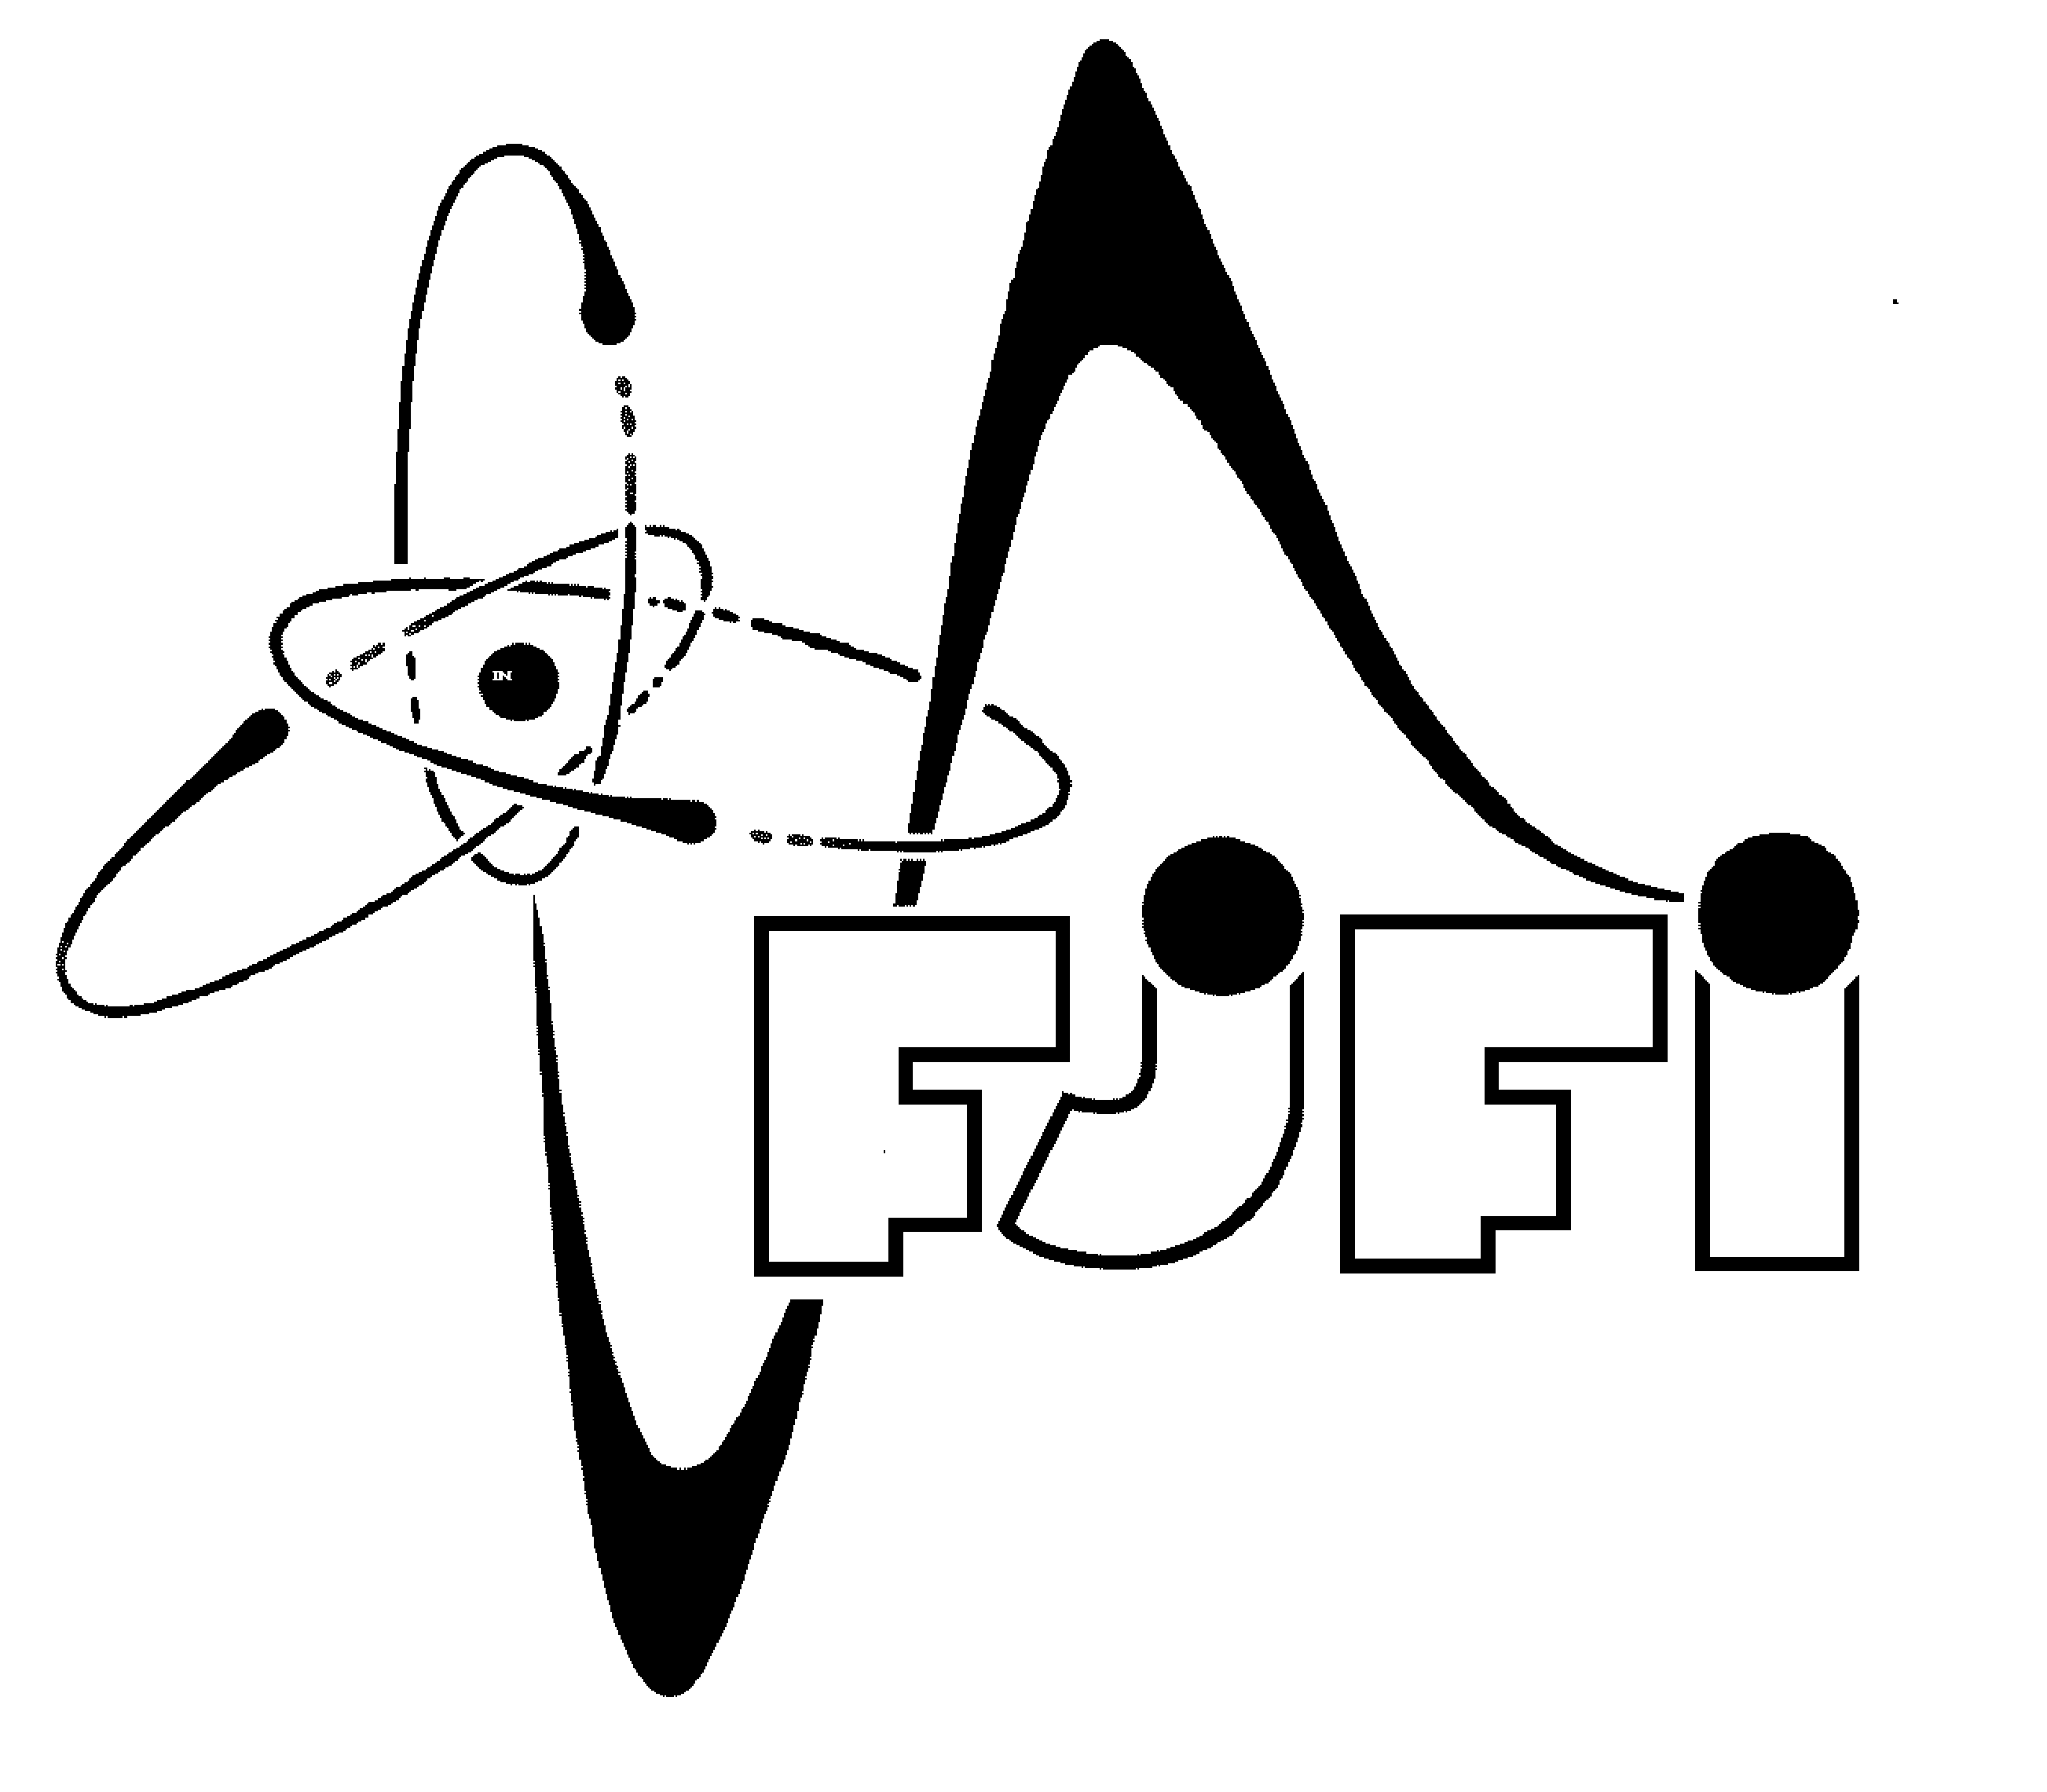
\includegraphics[width=0.2\textwidth]{Images/TITLE/fjfi}\\[1cm] % Include a department/university logo - this will require the graphicx package	
	
%	\noindent %
%	\begin{minipage}[c]{3cm}%
%		\noindent \begin{center}
%			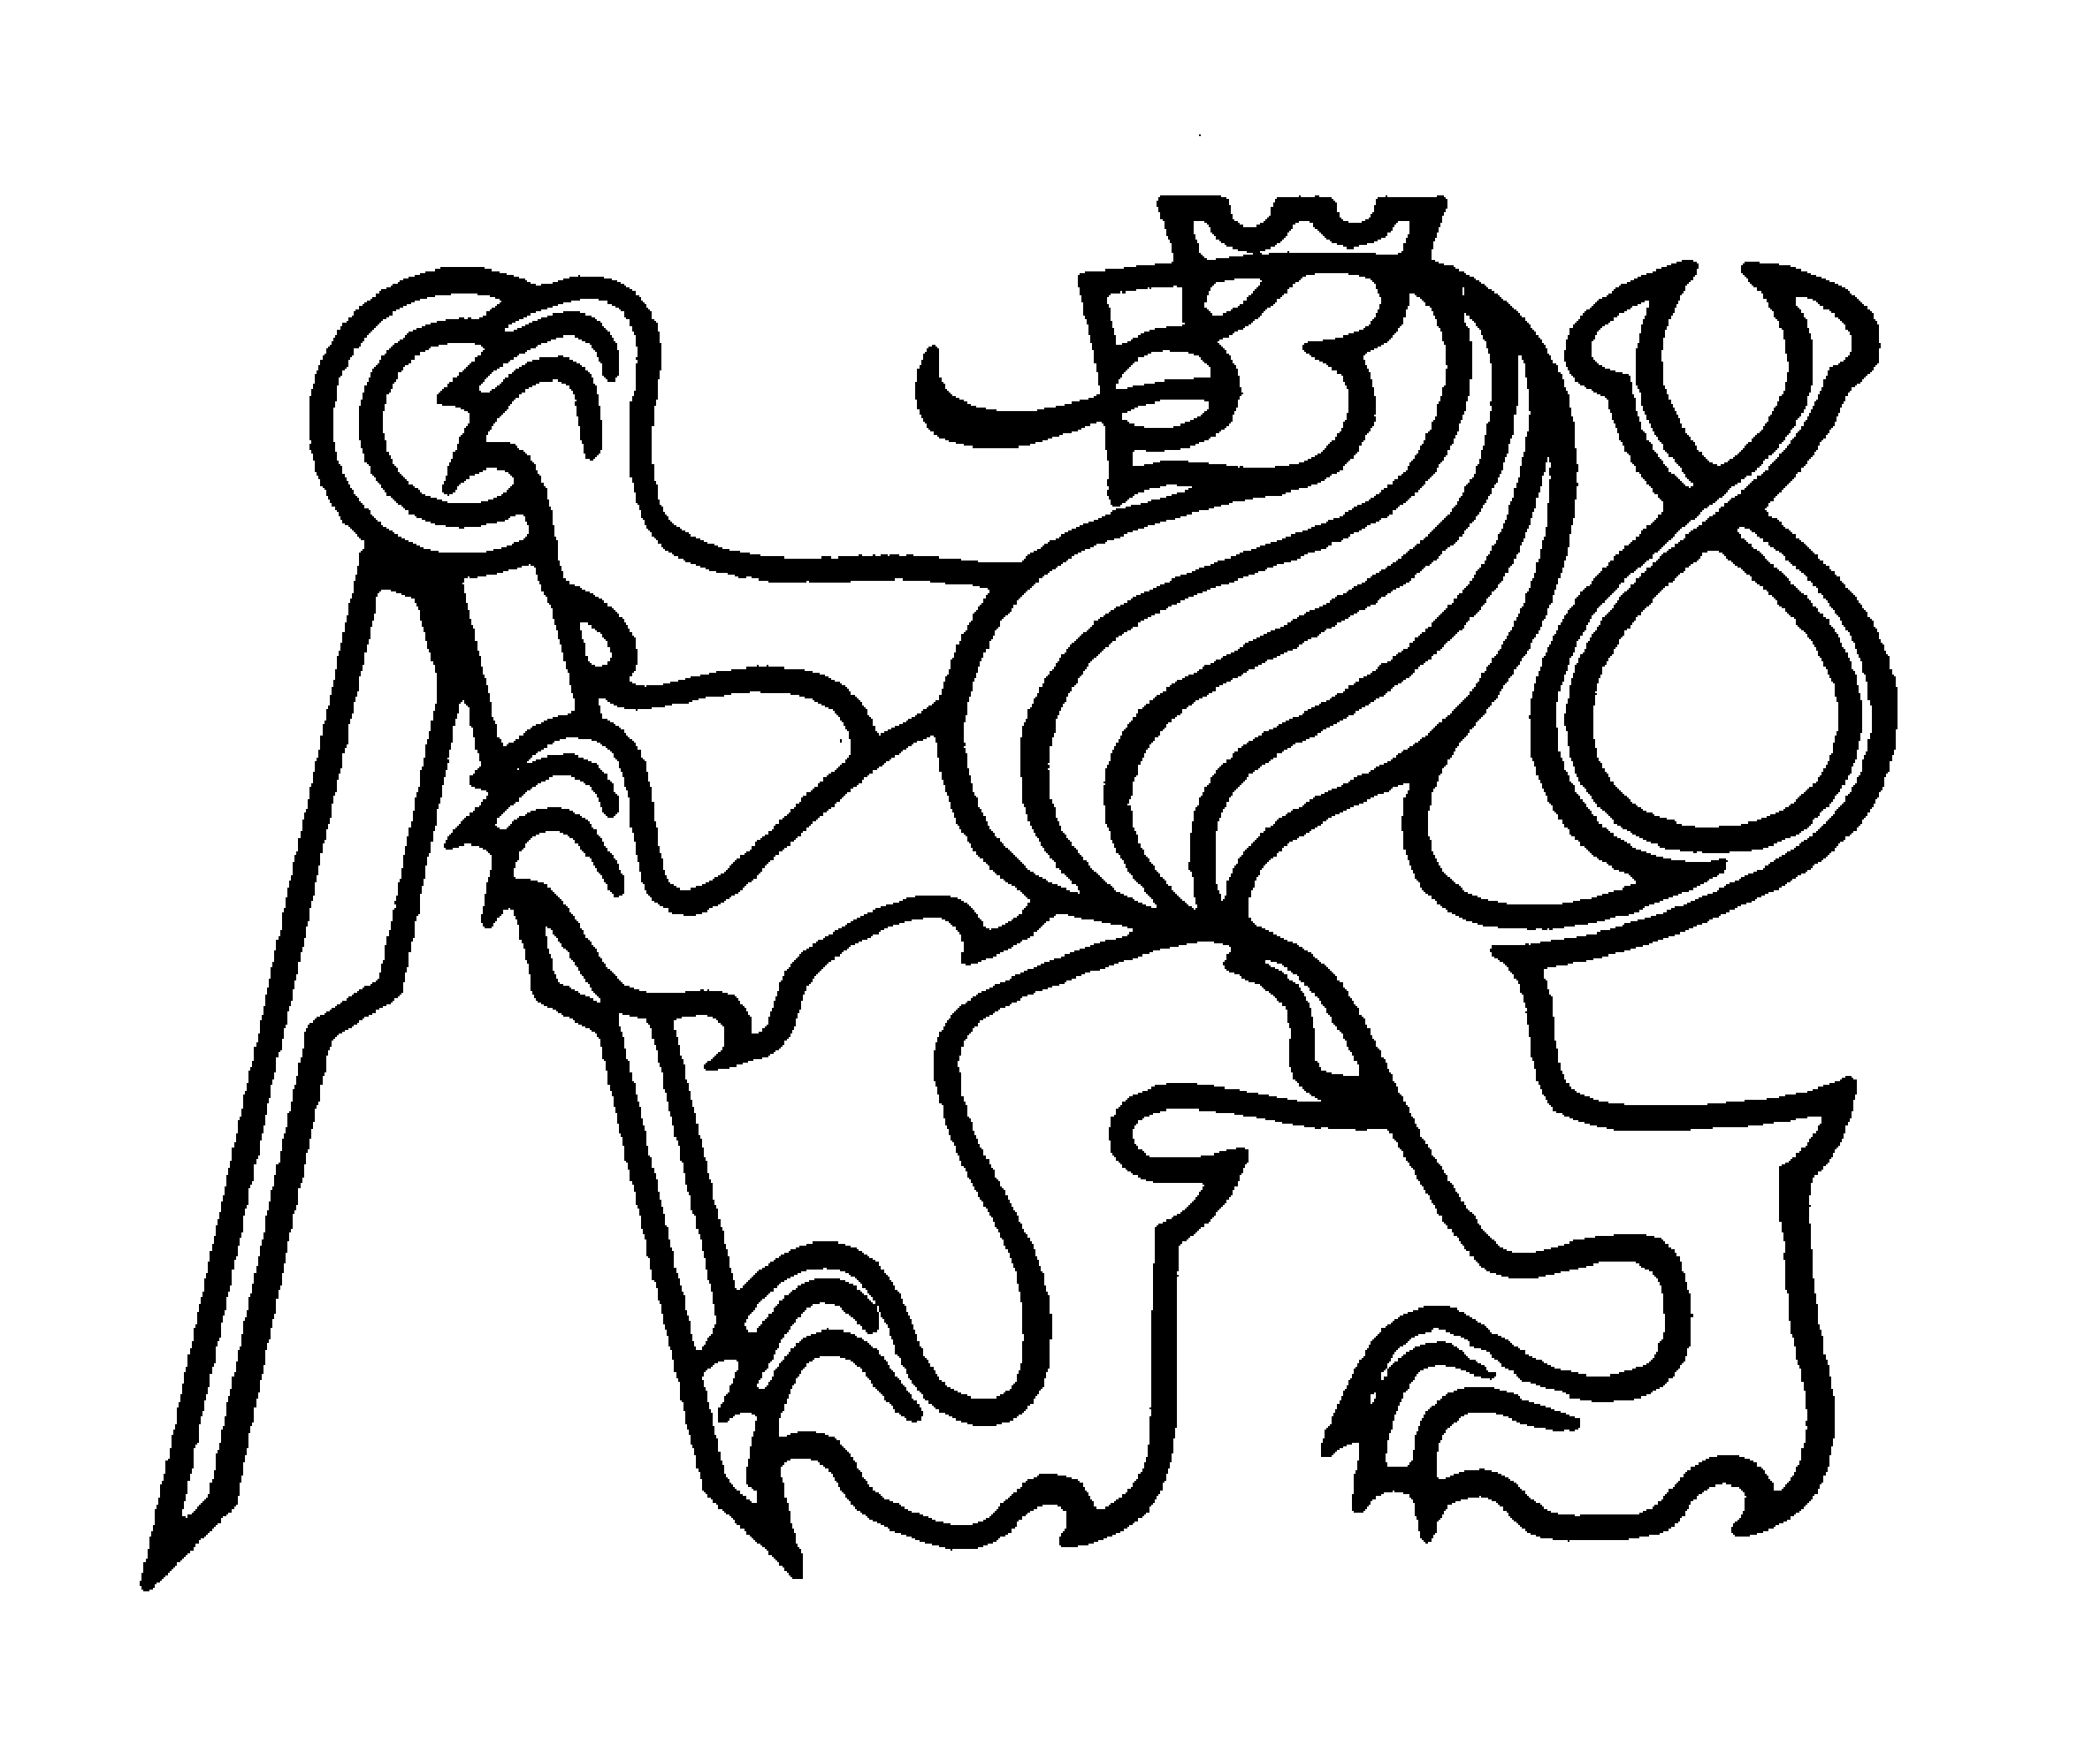
\includegraphics[width=3cm,height=3cm,keepaspectratio]{Images/TITLE/cvut}
%			\par\end{center}%
%	\end{minipage}%
%	\begin{minipage}[c]{0.6\linewidth}%
%		\begin{center}
%			\textsc{\large{}České vysoké učení technické v Praze}{\large{}}\\
%			{\large{}Fakulta jaderná a fyzikálně inženýrská}
%			\par\end{center}%
%	\end{minipage}%
%	\begin{minipage}[c]{3cm}%
%		\noindent \begin{center}
%		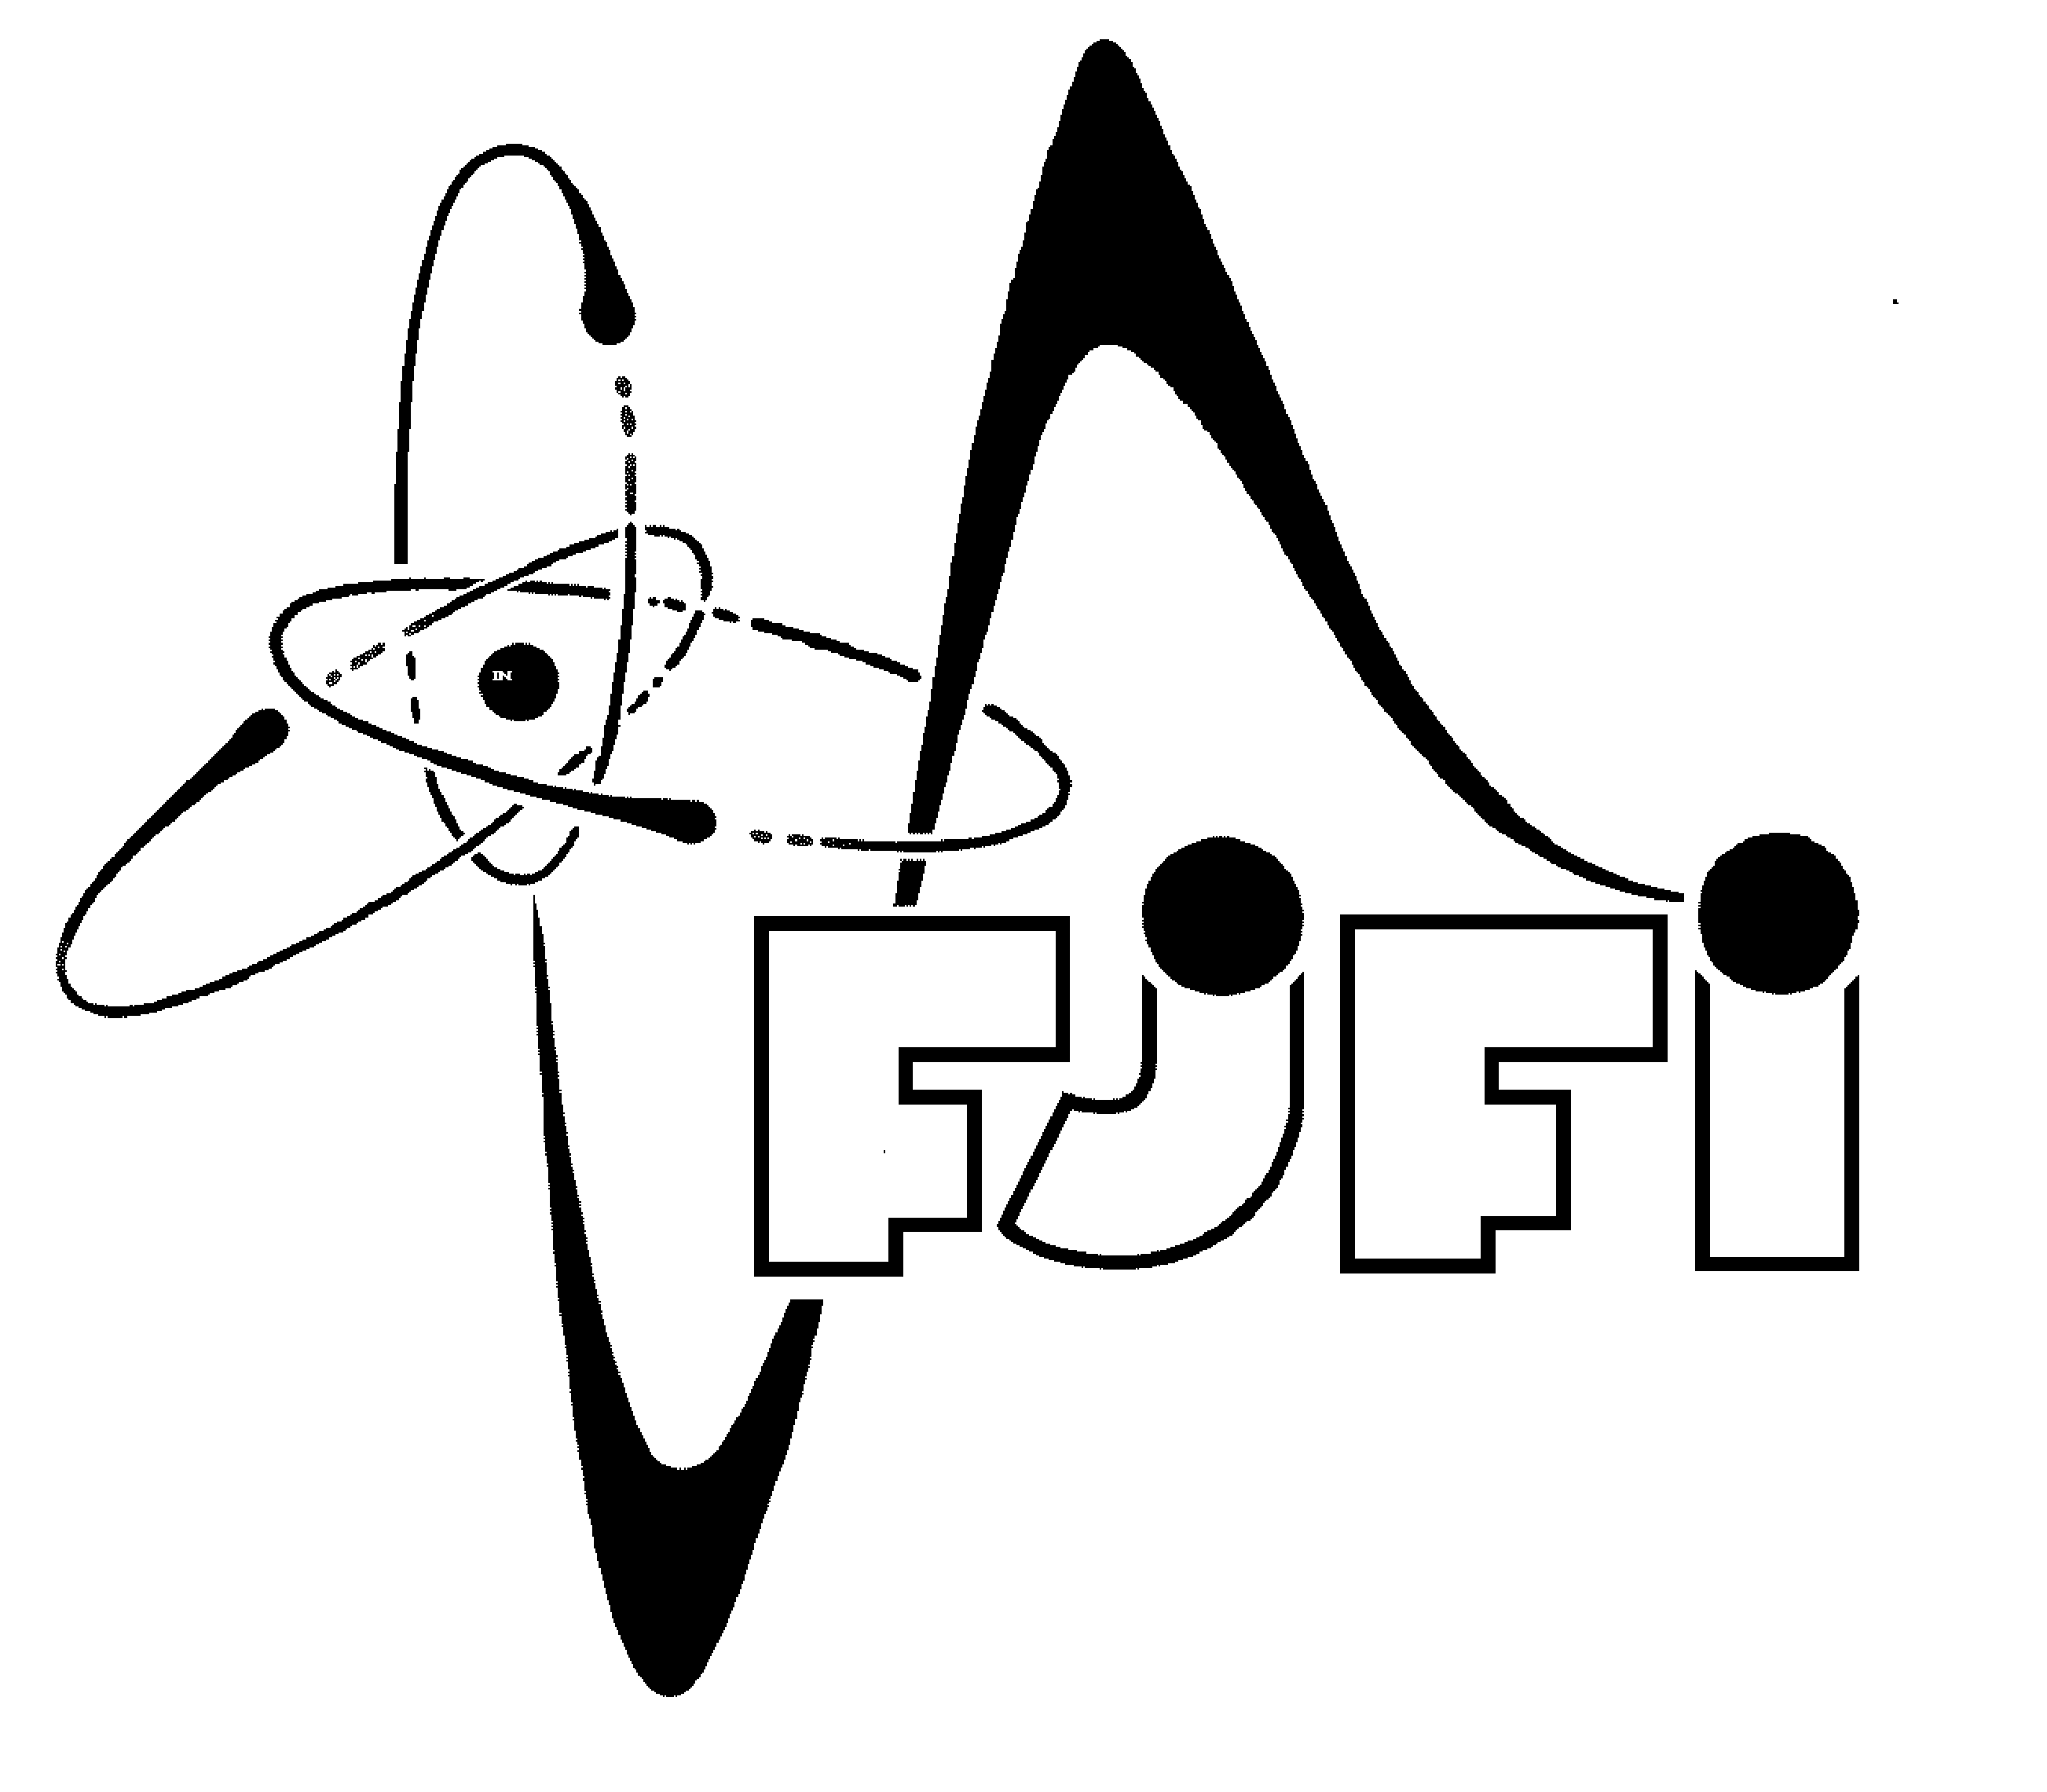
\includegraphics[width=3cm,height=3cm,keepaspectratio]{Images/TITLE/fjfi}
%		\par\end{center}%
%	\end{minipage}
%	\vspace{3cm}
	
	\textsc{\Large ASM}\\[0.5cm] % Major heading such as course name
	\textsc{\large Dataset n.6}\\[0.5cm] % Minor heading such as course title
	\HRule\\[0.4cm]
	{\huge\bfseries Fitting Percentage of Body Fat to Simple Body Measurements}\\[0.4cm] % Title of your document
	\HRule\\[1.5cm]
	{\large\textit{Author:}}\\
	Vladislav \textsc{Belov}\\
	\vfill\vfill\vfill\vfill\vfill\vfill\vfill % Position the date 3/4 down the remaining page
	{\large\today} % Date, change the \today to a set date if you want to be precise
	
	%------------------------------------------------
	%	Logo
	%------------------------------------------------
	
%	\vfill\vfill
%	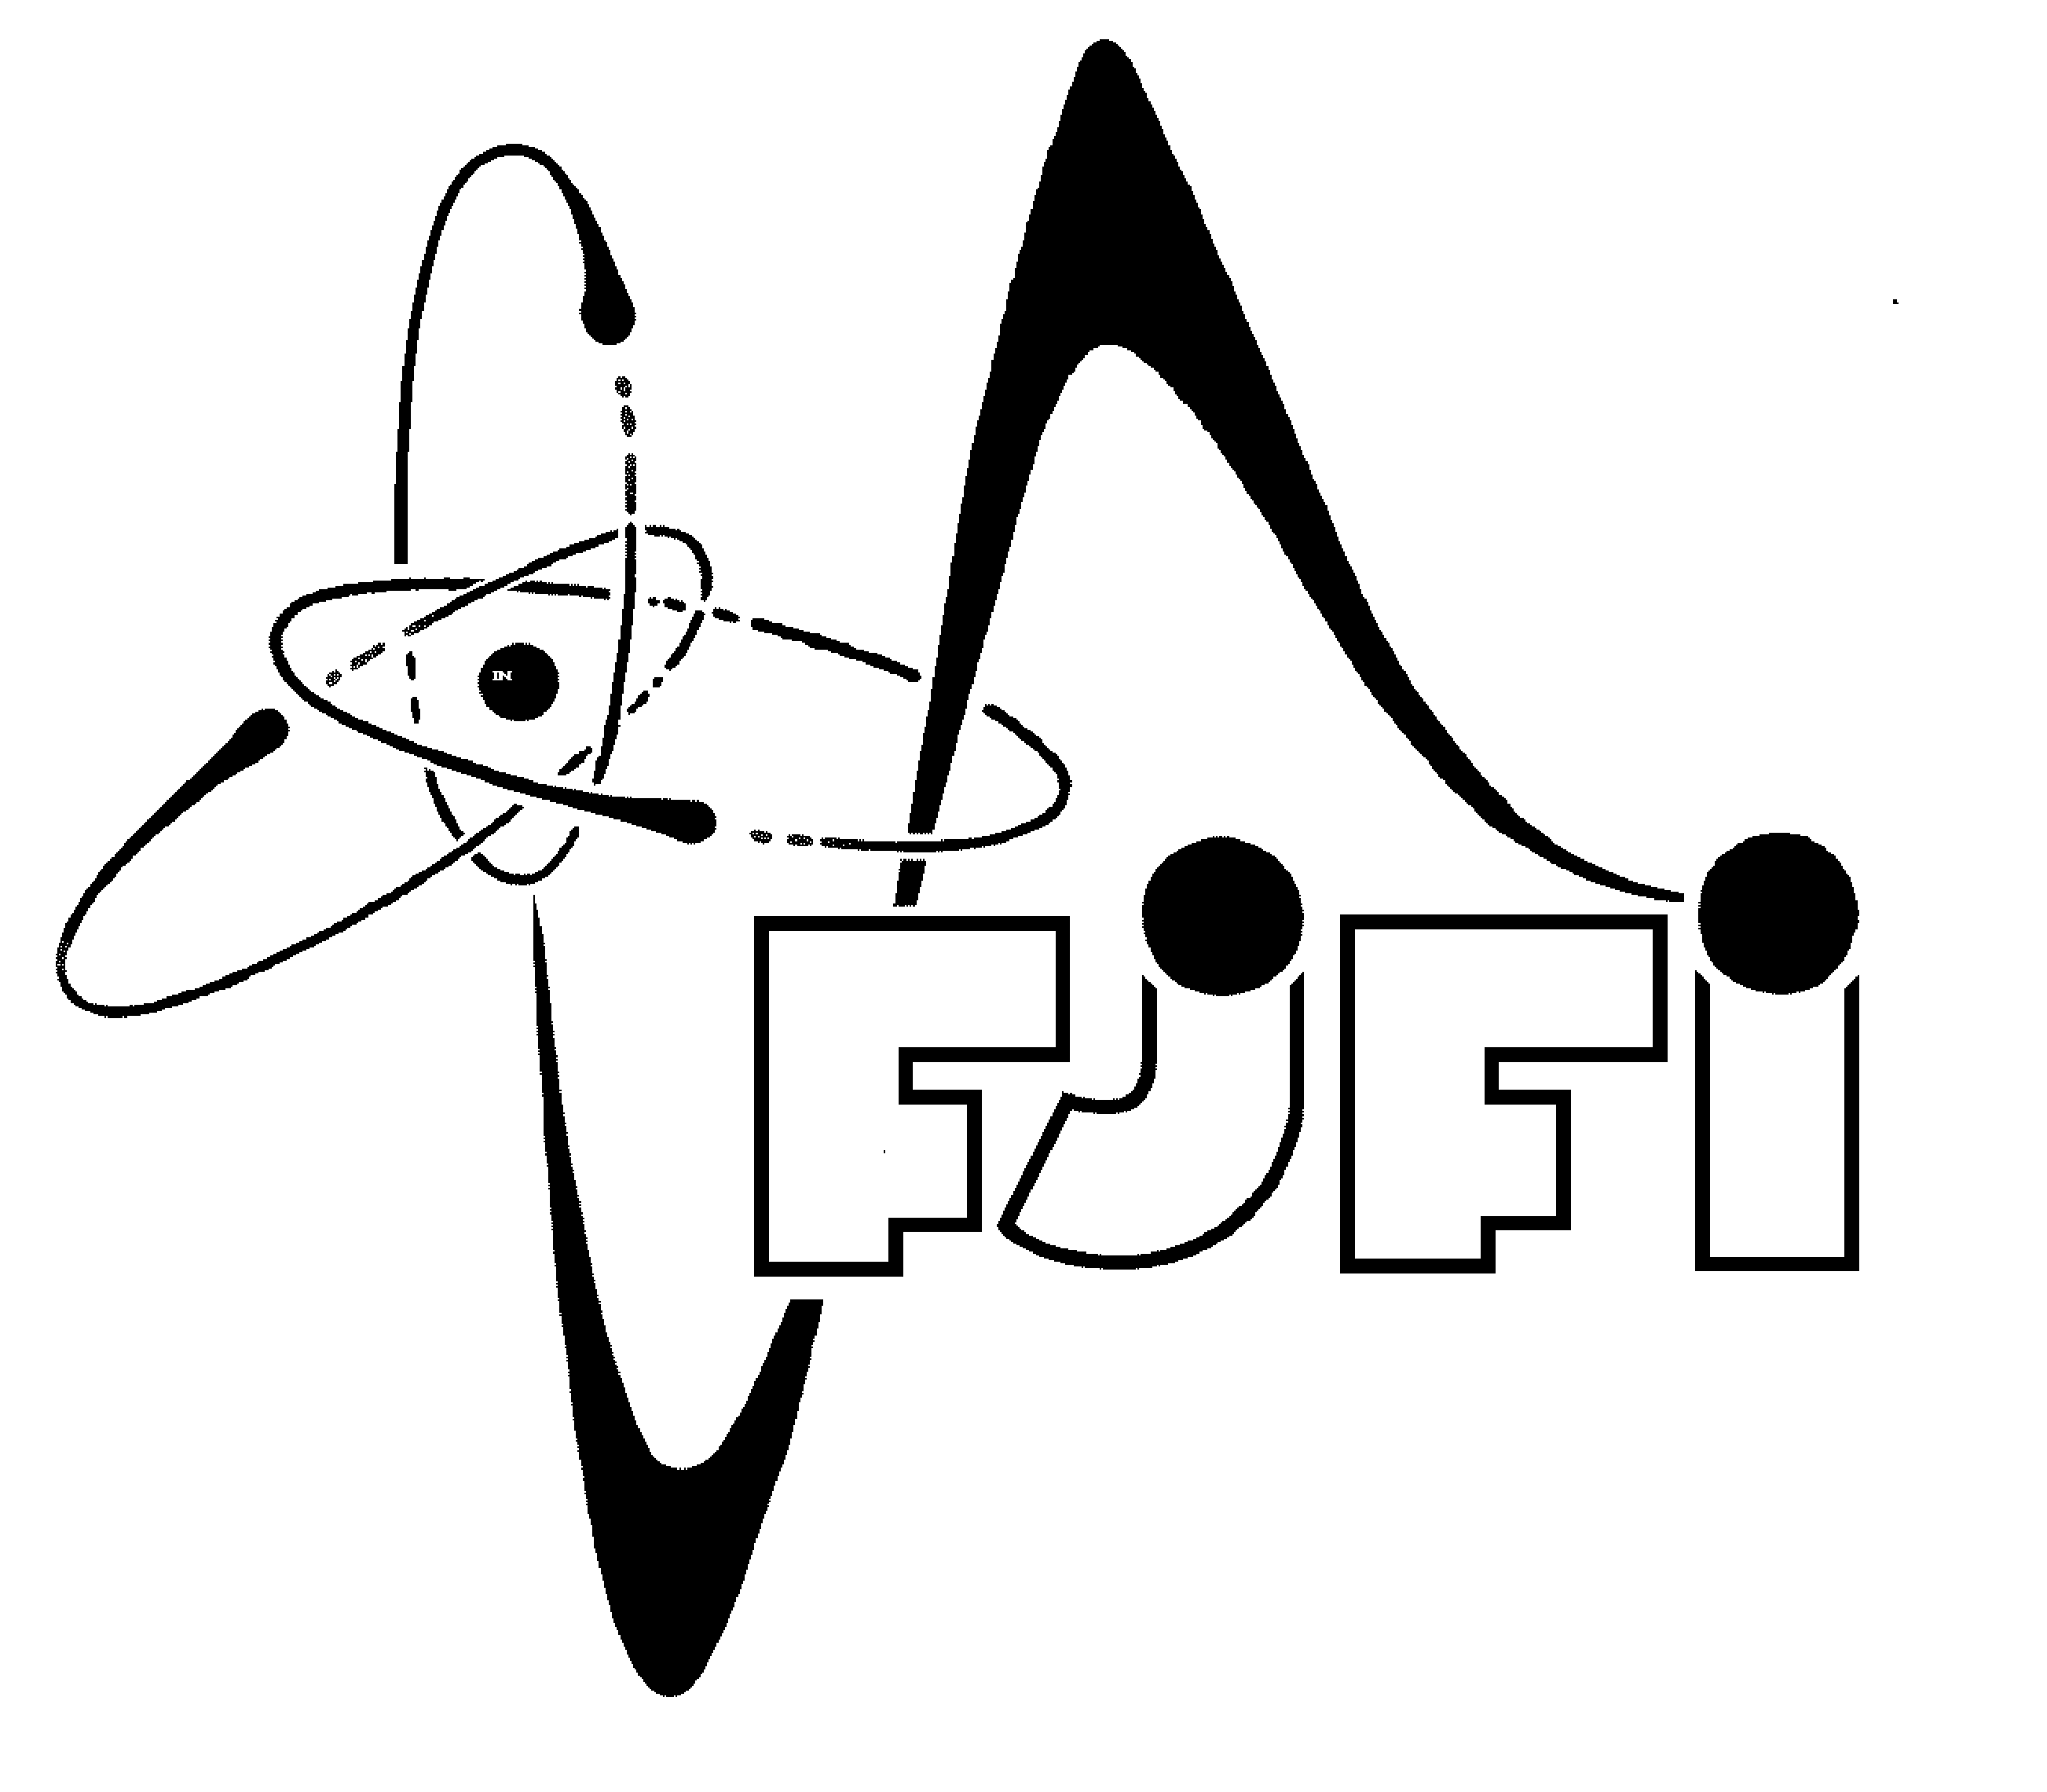
\includegraphics[width=0.2\textwidth]{Images/TITLE/fjfi}\\[1cm] % Include a department/university logo - this will require the graphicx package
%	
	%----------------------------------------------------------------------------------------
	
	\vfill % Push the date up 1/4 of the remaining page
	
\end{titlepage}

%\tableofcontents
%\newpage{}

\section{Outline}\label{sec:outline}

In this paper we will perform an analysis of the dataset which contains simple measurements of $252$ men. Circumferences of body parts, age, weight and fat percentage are a part of the dataset. After providing descriptive statistics in section \ref{sec:desc} and performing a more detailed examination of some selected variables in section \ref{sec:analysis}, we will attempt to fit percentage of body fat to some of the body measurements in section \ref{sec:regression}. Body fat percentage can be measured using either Siri's equation or Brozek's equation:

\begin{equation*}
	\begin{split}
		\text{Siri: } \, &\frac{457}{\text{Body Density}} - 414.2,	\\ \\
		\text{Brozek: } \, &\frac{495}{\text{Body Density}} - 450.
	\end{split}
\end{equation*}

\section{Descriptive Statistics}\label{sec:desc}

\subsection{Numerical Analysis of Selected Variables}

In this section a general numerical overview of the dataset population is be provided. Basic information about population's weight and height is available in Tab.~\ref{tab:desc1}. Age is also considered a continuous instance, nevertheless, for illustrative purposes we have categorized it, and results can be seen in Tab.~\ref{tab:desc2}.\footnote{Inches were converted to centimeters, pounds to kilograms.} 

\medskip

\begin{table}[ht!]
	\centering
	\begin{tabular}{|c||c|c|c|c|c|c|}
		\hline 
		Variable &  Min. Value &  1st Quantile &  Median &  Mean Value &  3rd Quantile & Max. Value   \\ 
		\hline \hline 
		Total Weight, [kg] & 53.75 & 72.12 & 80.06 & 81.16 & 89.36 & 164.72   \\ 
		\hline 
		Fat-Free Weight, [kg] & 48.04 & 59.58 & 64.21 & 65.19 & 69.8 & 109.09   \\ 
		\hline 
		Height, [cm] & 74.93 & 173.35 & 177.8 & 178.18 & 183.51 & 197.49   \\ 
		\hline 
	\end{tabular} 
	\caption{Numerical descriptive statistics for weight and height of the population.}	
	\label{tab:desc1}
\end{table}

\begin{table}[ht!]
	\centering
	\begin{tabular}{|c||c|c|}
		\hline 
		Age & Count &  \%   \\ 
		\hline \hline 
		22-34 & 53 & 21.03   \\
		\hline
		35-49 & 116 & 46.03  \\
		\hline  
		50-64 & 62 &  24.6  \\
		\hline 
		65-81 & 21 &  8.34  \\
		\hline 
	
	\end{tabular} 
	\caption{Contingency table for age.}
	\label{tab:desc2}	
\end{table}
 
\subsection{Graphical Analysis of Selected Variables}

\subsection{Fat Percentage Analysis}

As body fat percentage is heavily dependent of body density, this section is opened by the histogram of it, see Fig.~\ref{fig:body_density_histogram}. Observing this diagram, we can speculate, that men with higher body weight have bodies with less density. Another noteworthy observation is that the histogram resembles normal distribution (Fig.~\ref{fig:density_fitdist}). However, more detailed analysis of this fact is provided in section \ref{sec:analysis}.

\medskip

In Fig.~\ref{fig:fat_percentage_boxplot} one can see the comparative diagram of both Siri's and Brozek's equations results. Similarities between them start to become noticeable. Looking at comparison of cumulative distribution functions (see Fig.~\ref{fig:cdf_brozek_siri}), we can speculate, that they have similar distributions and, moreover, those distributions are normal, the fit is available in Fig.~\ref{fig:brozek_fitdist}-\ref{fig:siri_fitdist}. Relevant tests are carried out in section \ref{sec:analysis}.

\newpage

\vspace*{\fill}
\begin{figure}[H]
	\centering
	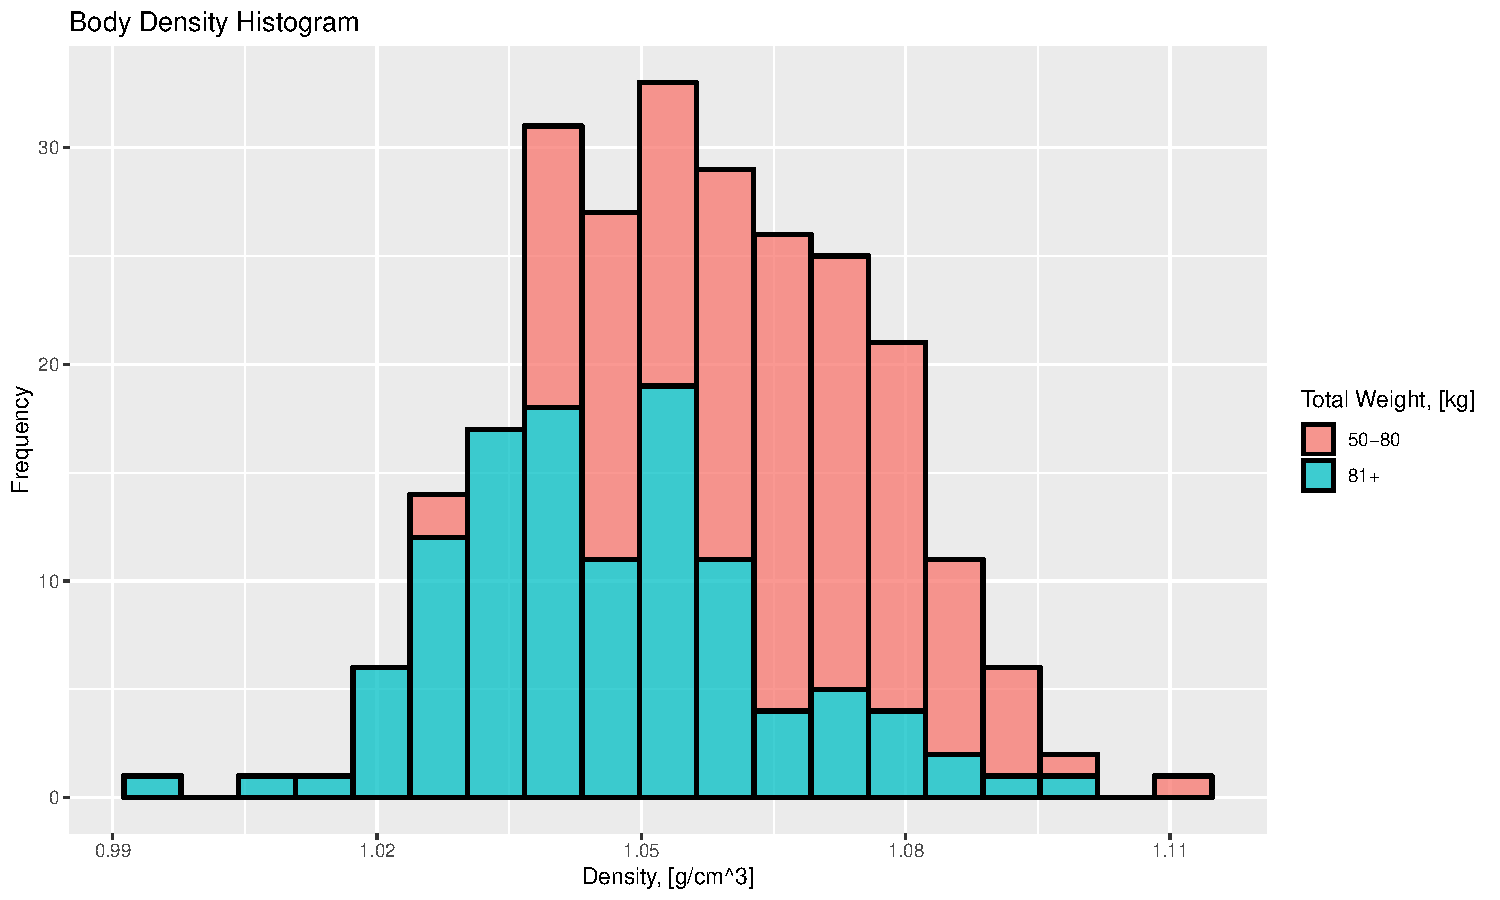
\includegraphics[width=0.75\linewidth]{Images/FIGURES/body_density_histogram}
	\caption{Body density histogram with categorized total weight for illustrative purposes.}
	\label{fig:body_density_histogram}
\end{figure}

\begin{figure}[H]
	\centering
	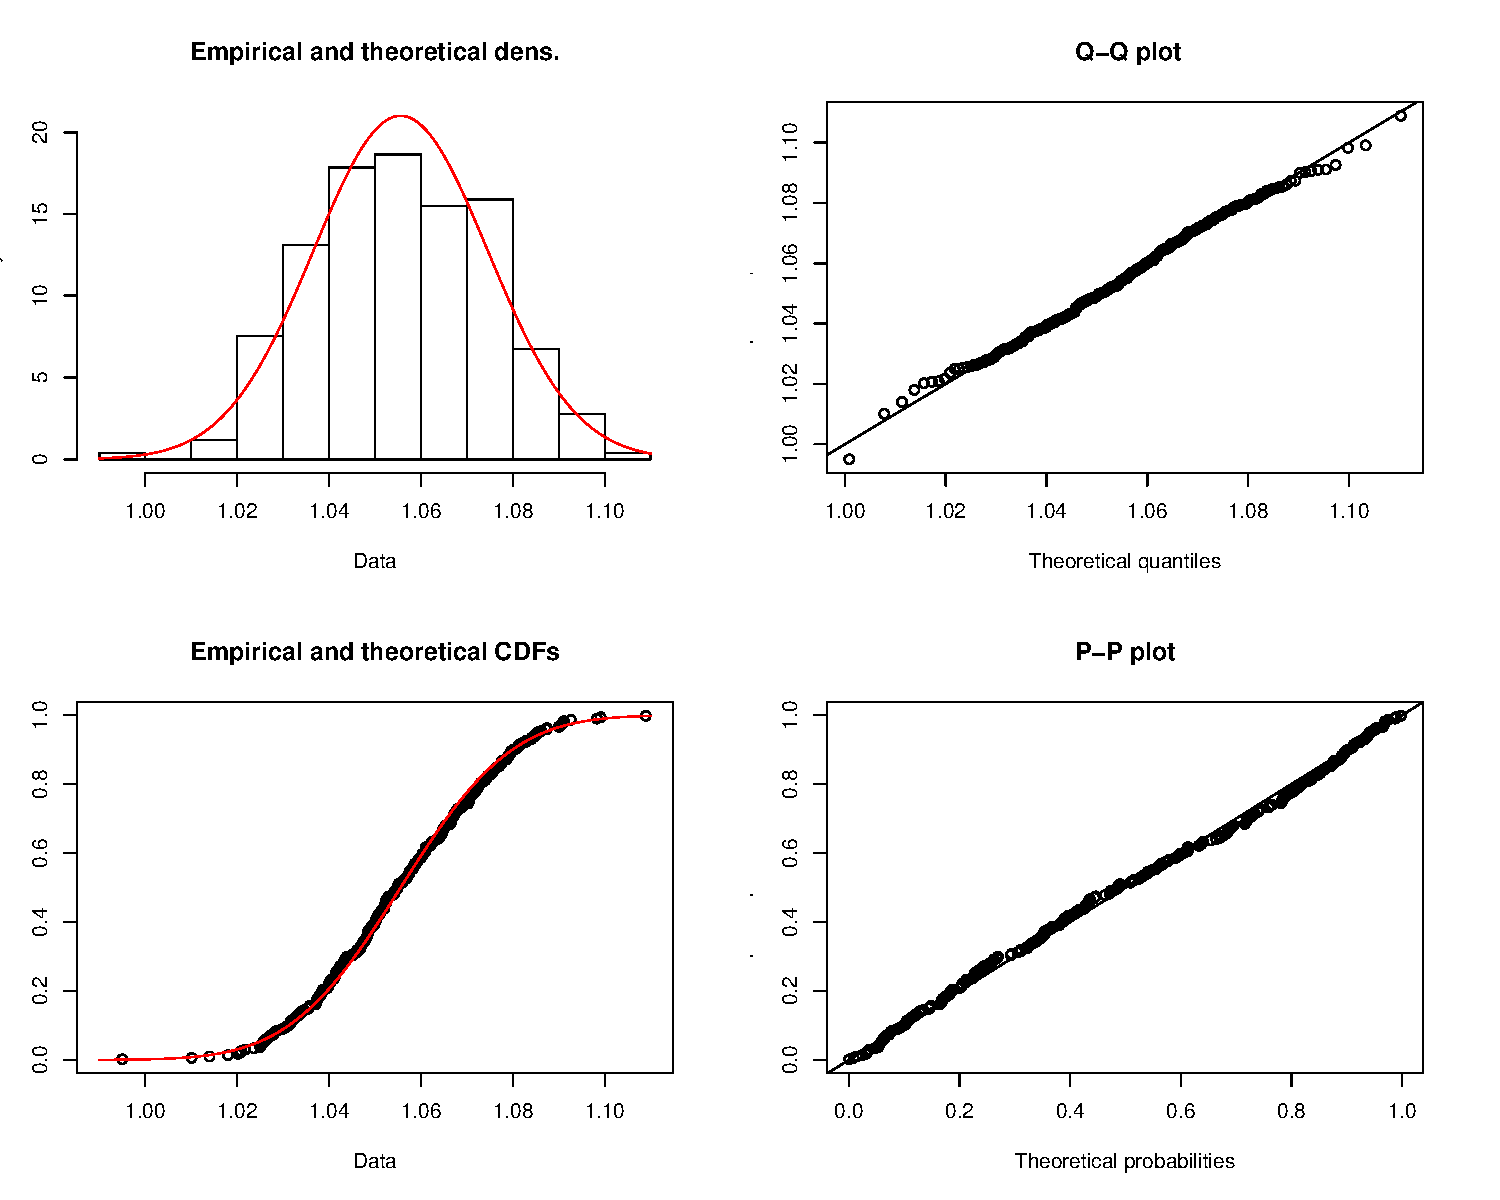
\includegraphics[width=0.8\linewidth]{Images/FIGURES/density_fitdist}
	\caption{Normal distribution fit for body density.}
	\label{fig:density_fitdist}
\end{figure}
\vspace*{\fill}

\newpage

\begin{figure}[H]
	\centering
	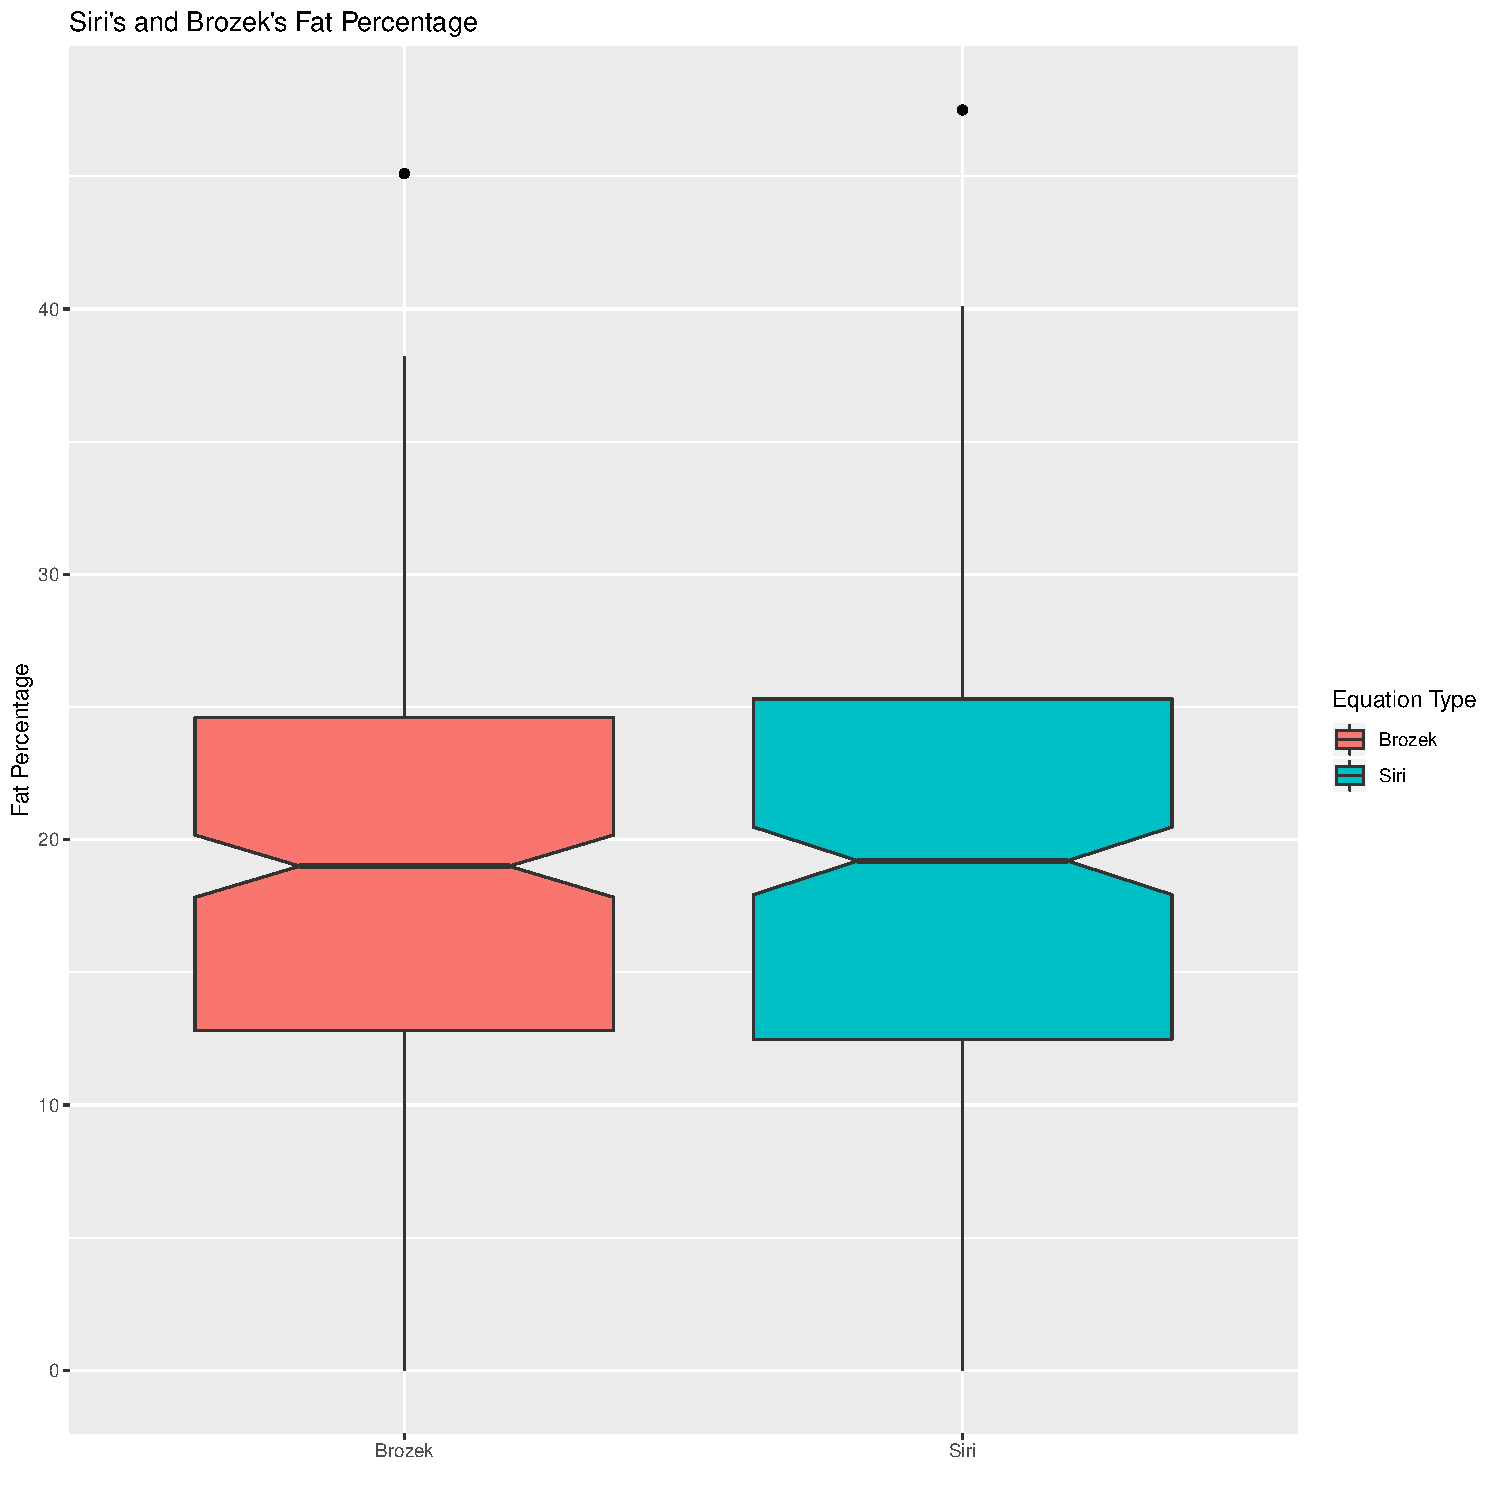
\includegraphics[width=0.7\linewidth]{Images/FIGURES/fat_percentage_boxplot}
	\caption{Comparative box plot of Siri's and Brozek's equations results.}
	\label{fig:fat_percentage_boxplot}
\end{figure}

\begin{figure}[H]
	\centering
	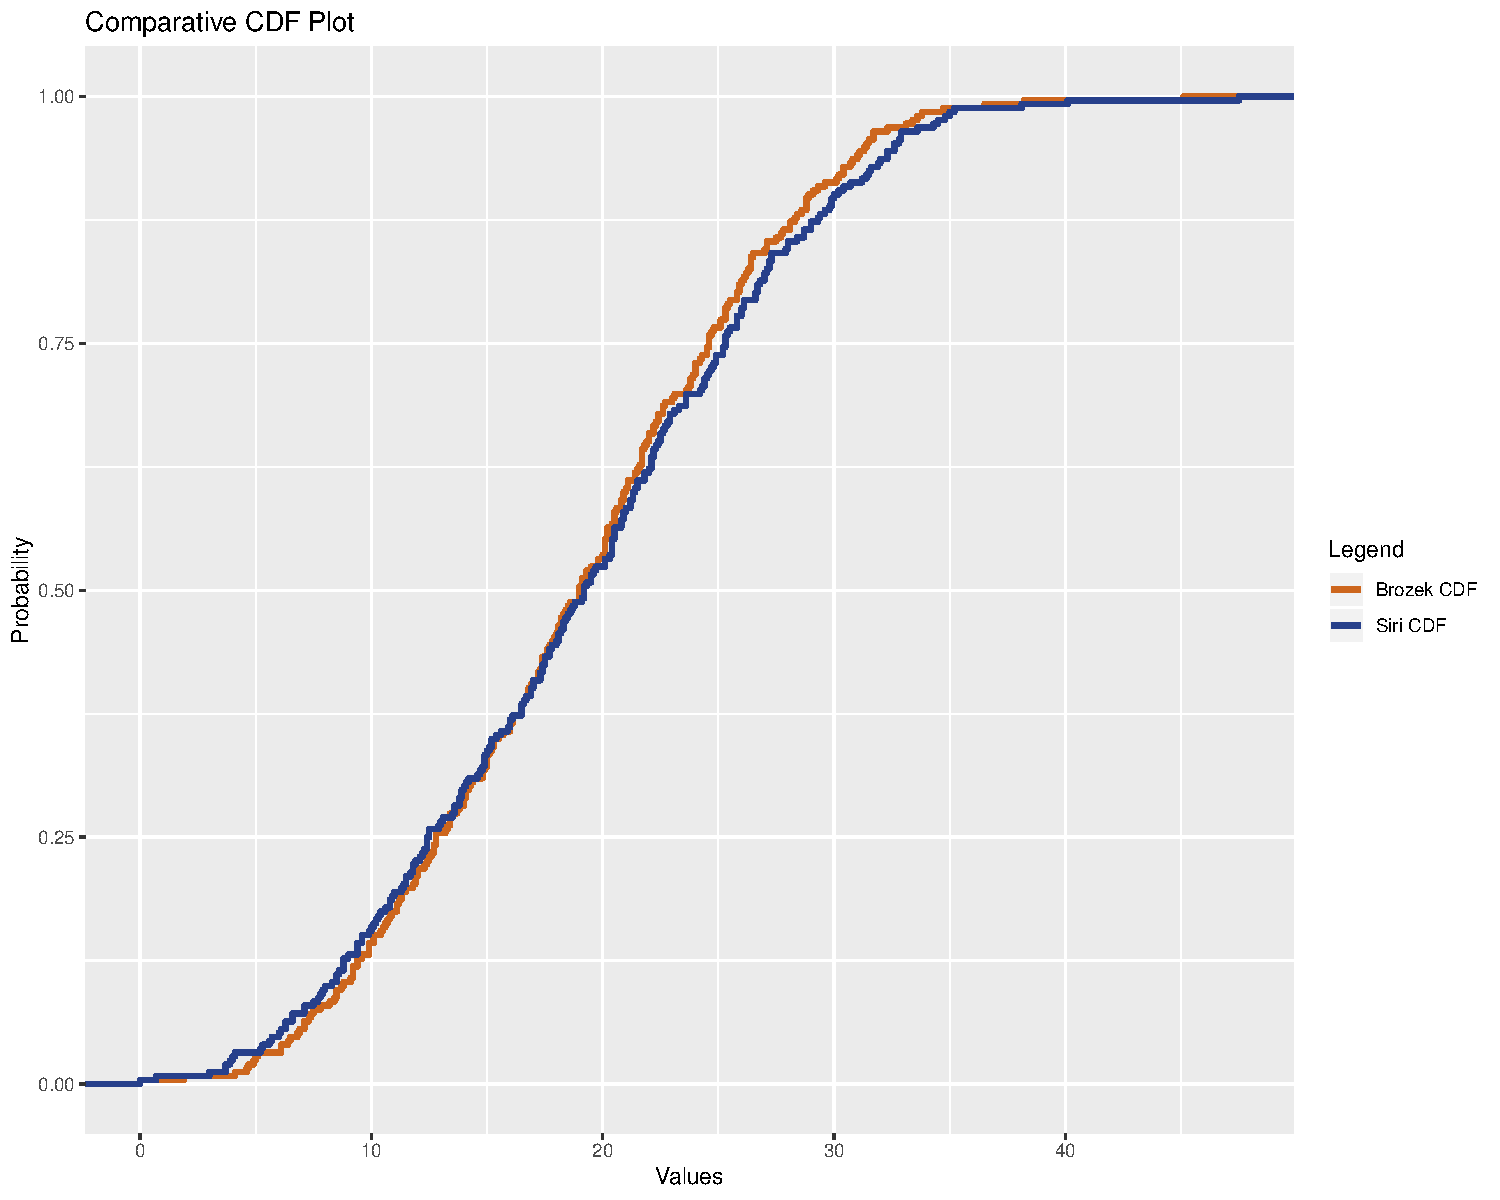
\includegraphics[width=0.75\linewidth]{Images/FIGURES/cdf_brozek_siri}
	\caption{Comparative plot of cumulative distribution functions for Siri's and Brozek's equations results.}
	\label{fig:cdf_brozek_siri}
\end{figure}

\newpage

\vspace*{\fill}
\begin{figure}[H]
	\centering
	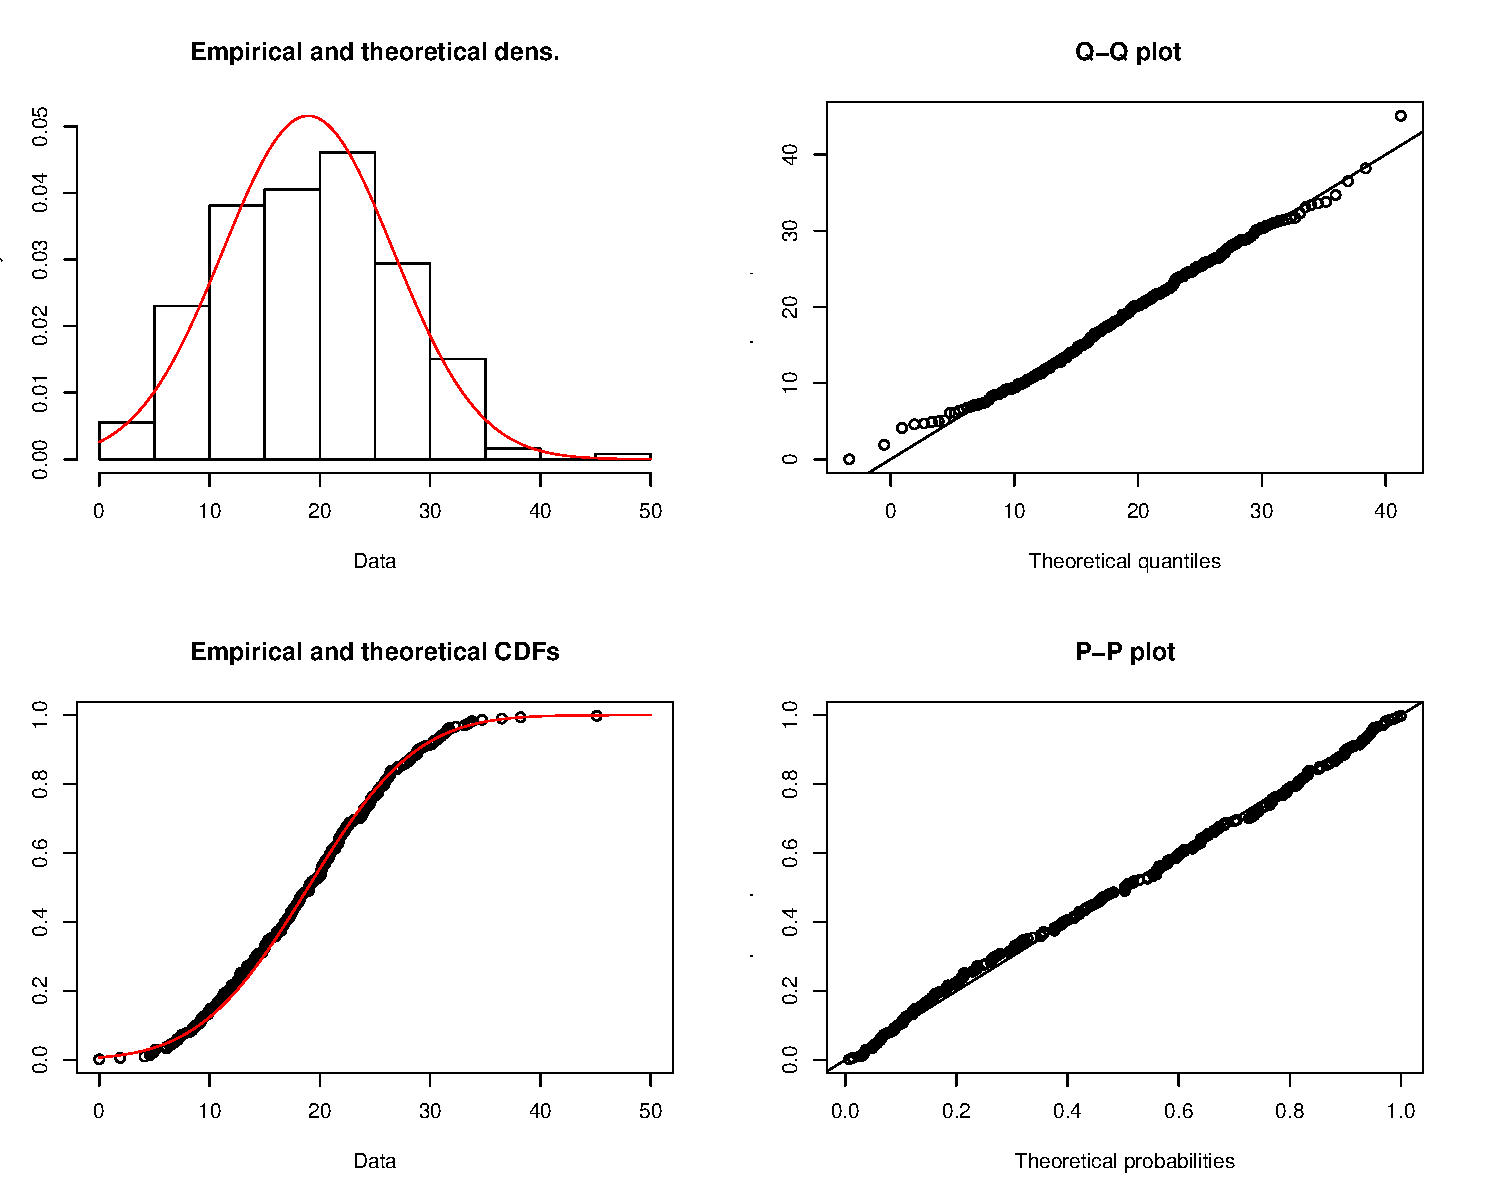
\includegraphics[width=0.8\linewidth]{Images/FIGURES/brozek_fitdist}
	\caption{Normal distribution fit for Brozek's equation results.}
	\label{fig:brozek_fitdist}
\end{figure}

\begin{figure}[H]
	\centering
	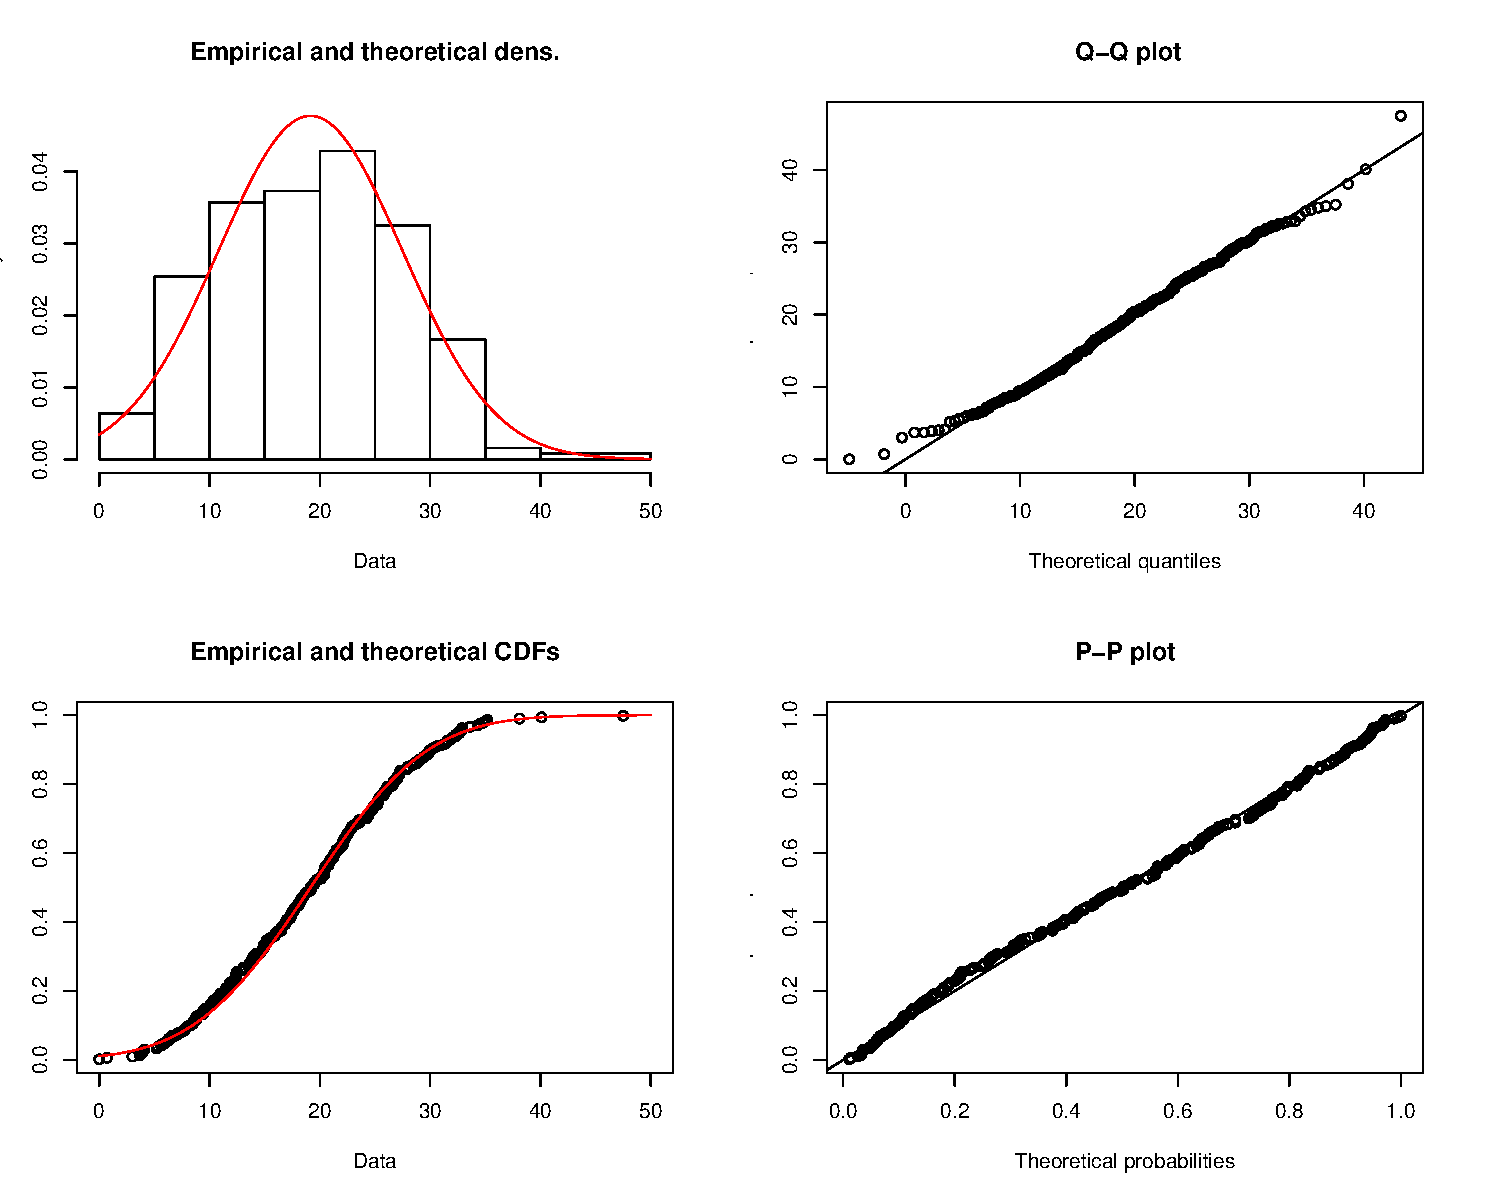
\includegraphics[width=0.8\linewidth]{Images/FIGURES/siri_fitdist}
	\caption{Normal distribution fit for Siri's equation results.}
	\label{fig:siri_fitdist}
\end{figure}
\vspace*{\fill}

\newpage


\subsection{Total Body Weight Scatter Plots}

In this section we will look at the behavior of total body weight in the scope of the provided dataset.


\begin{figure}[H]
	\centering
	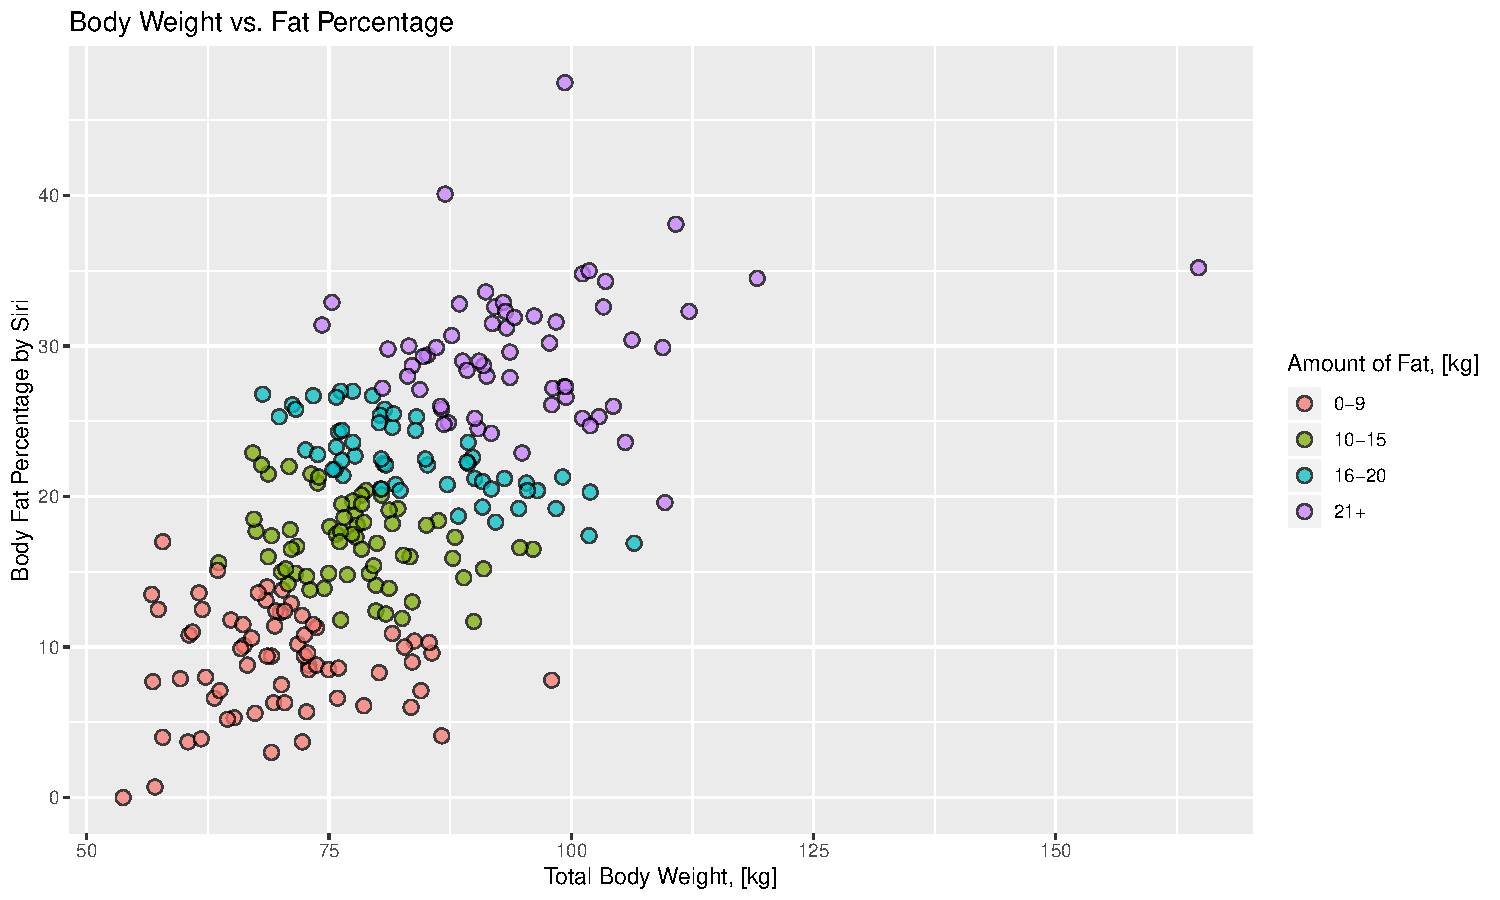
\includegraphics[width=1.0\linewidth]{Images/FIGURES/total_weight_vs_siri}
	\caption{Influence of total body weight on the body fat percentage.}
	\label{fig:total_weight_vs_siri}
\end{figure}


\begin{figure}[H]
	\centering
	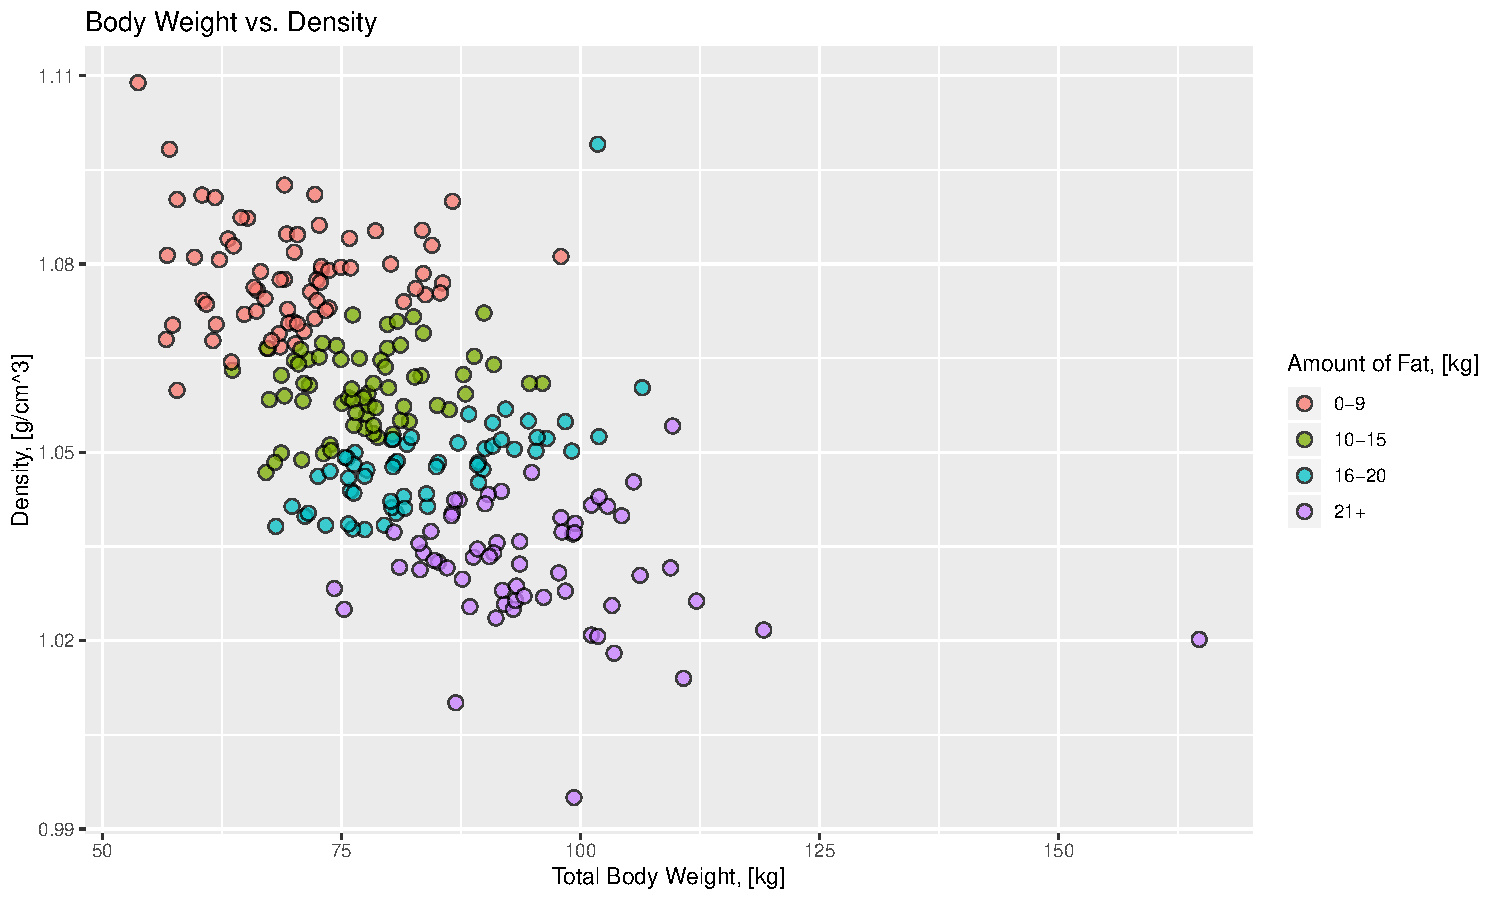
\includegraphics[width=1.0\linewidth]{Images/FIGURES/total_weight_vs_density}
	\caption{Influence of total body weight on body density.}
	\label{fig:total_weight_vs_density}
\end{figure}



%\begin{figure}[H]
%	\centering
%	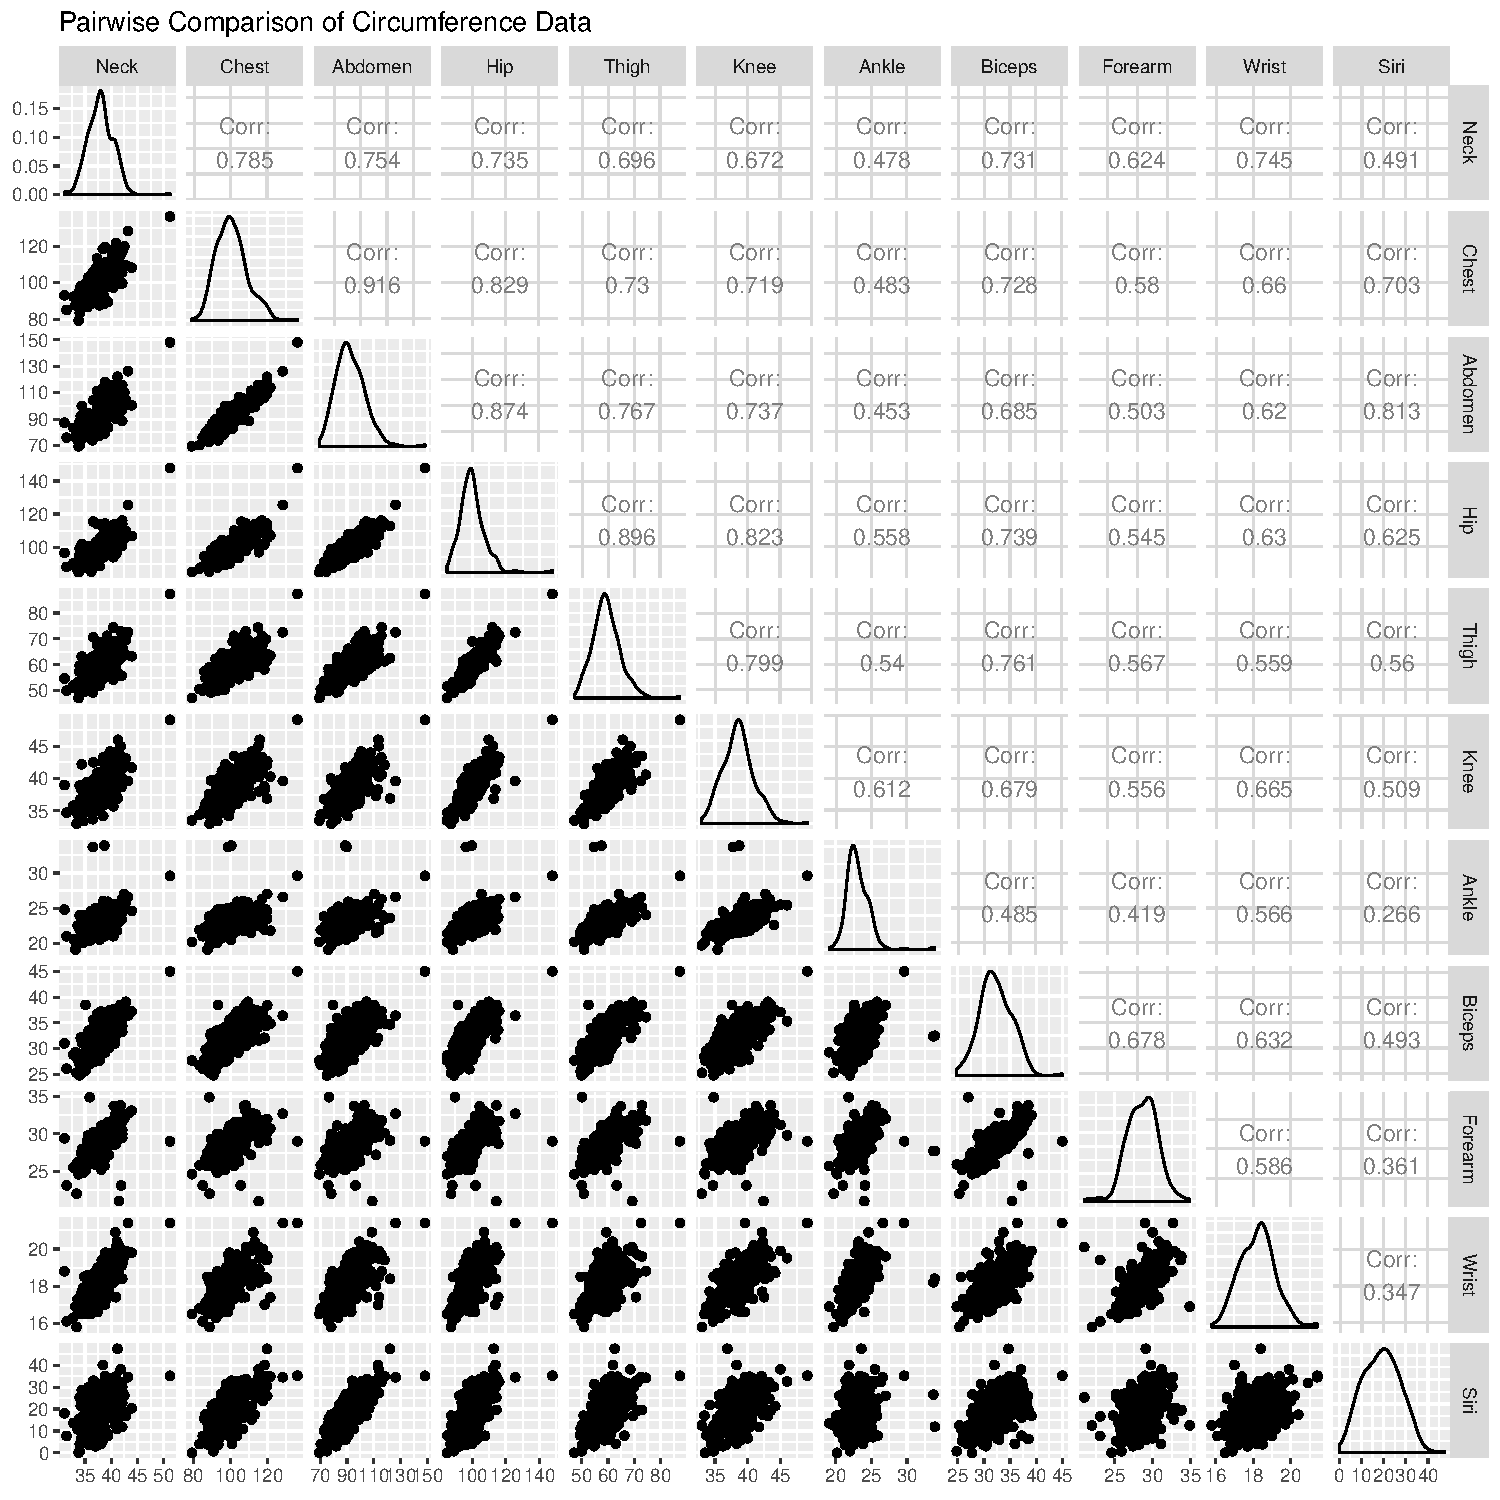
\includegraphics[width=1.0\linewidth]{Images/FIGURES/pairwise_comparison}
%	\caption{}
%	\label{fig:pairwise_comparison}
%\end{figure}


\newpage


\section{Data Analysis}\label{sec:analysis}


\newpage{}


\section{Multivariate Linear Regression}\label{sec:regression}

In the scope of this section we will consider observation $39$ with total weight equal to $164.7$ kg as an outlier and remove it from the dataset.

\subsection{2-variable Linear Regression}

In this section we will assume, that the results of Siri's equation can be explained by two variables: abdomen circumference and total weight. Then the linear model takes the following form, $\forall i \in \{1,2, \dots, 251\}$:

\begin{equation}
		Y_{i} = \beta_{0} + \beta_{1} X_{i,\,1} + \beta_{2} X_{i,\,2} + e_{i}
\end{equation}

\medskip
\noindent
which, with dropped mathematical notation for the response and explanatory variables, results in

\begin{equation*}
	\text{(Body Fat Percentage by Siri)} = \beta_{0} + \beta_{1} \cdot (\text{Abdomen CC}) + \beta_{2} \cdot (\text{Total Weight}).
\end{equation*}

\medskip

Results of the estimation can be observed in the table below. The value of the R-squared statistic is equal to $0.72$. This indicates, that $72\%$ of the variability of the response data is explained around its mean which is quite adequate for our purposes. 

\begin{table}[H]
	\centering
	\begin{tabular}{|c||c||c|c|}
		\hline 
		Parameter &  Estimated Value & \multicolumn{2}{c|}{Confidence Interval, $95\%$}  \\ 
		\hline \hline 
		Intercept, $\beta_{0}$ & -47.67 & -52.86 &  -42.48 \\ 
		\hline 
		Abdomen CC, $\beta_{1}$ & 0.98 & 0.87 &  1.09 \\ 
		\hline 
		Total Weight, $\beta_{2}$ & -0.29 & -0.38 & -0.2 \\ 
		\hline 
	\end{tabular} 
\caption{Estimated values for the 2-variable linear regression.}
\end{table}

The fit function is displayed in Fig.~\ref{fig:3d_linear_regression}. As can be seen in the Fig.~\ref{fig:2var_linear_regression}, the residuals are distributed acceptably on the plane (see the first column of the figure), normal Q-Q plot also indicates normality of residuals. Assuredly, as normality of residuals is the absolute assumption to perform linear regression, a relevant test has to be performed to support this hypothesis.

\begin{equation*}
	\text{H}_{0}: res \in \{ \mathcal{N} (\mu,\,\sigma^{2}): \mu \in \mathbb{R}, \, \sigma^{2} > 0 \} \text{ vs. }
	\text{H}_{1}: res \not\in \{ \mathcal{N} (\mu,\,\sigma^{2}): \mu \in \mathbb{R}, \, \sigma^{2} > 0 \}
\end{equation*}

\medskip

According to the Lilliefors test with statistical significance set to $5\%$ we cannot reject the null hypothesis, as the p-value is equal to $0.33$.

\begin{figure}[H]
	\centering
	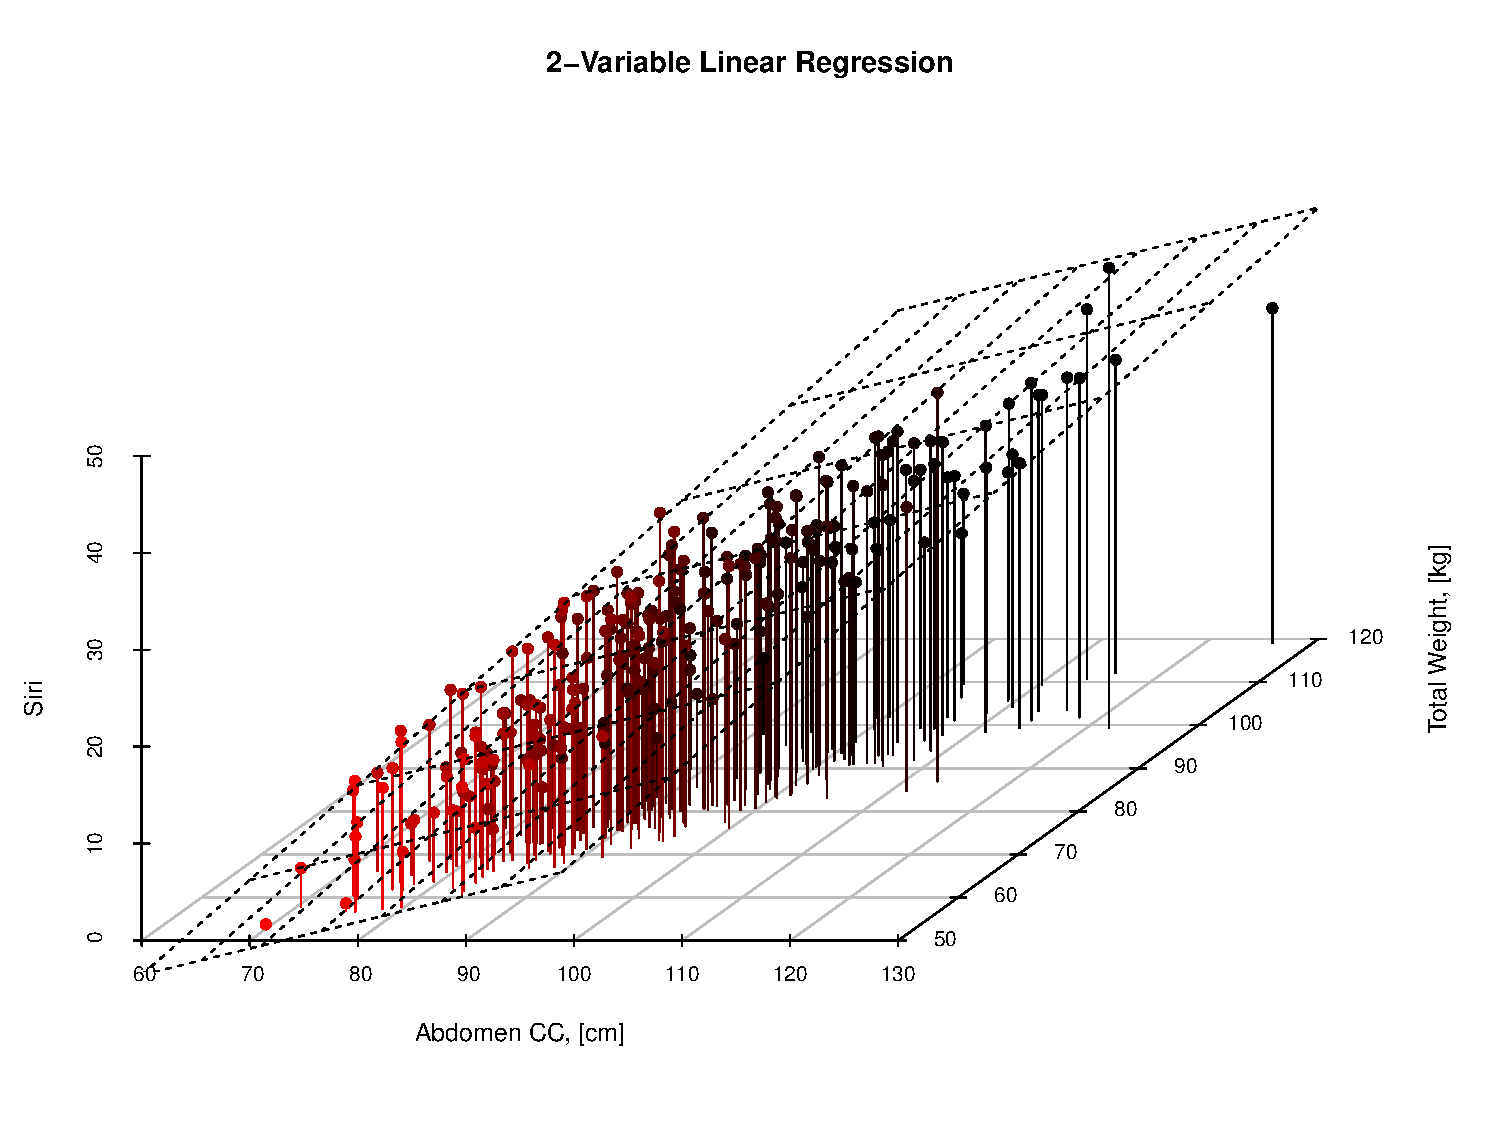
\includegraphics[width=0.75\linewidth]{Images/FIGURES/3d_linear_regression}
	\caption{Fit of the linear model.}
	\label{fig:3d_linear_regression}
\end{figure}

\begin{figure}[H]
	\centering
	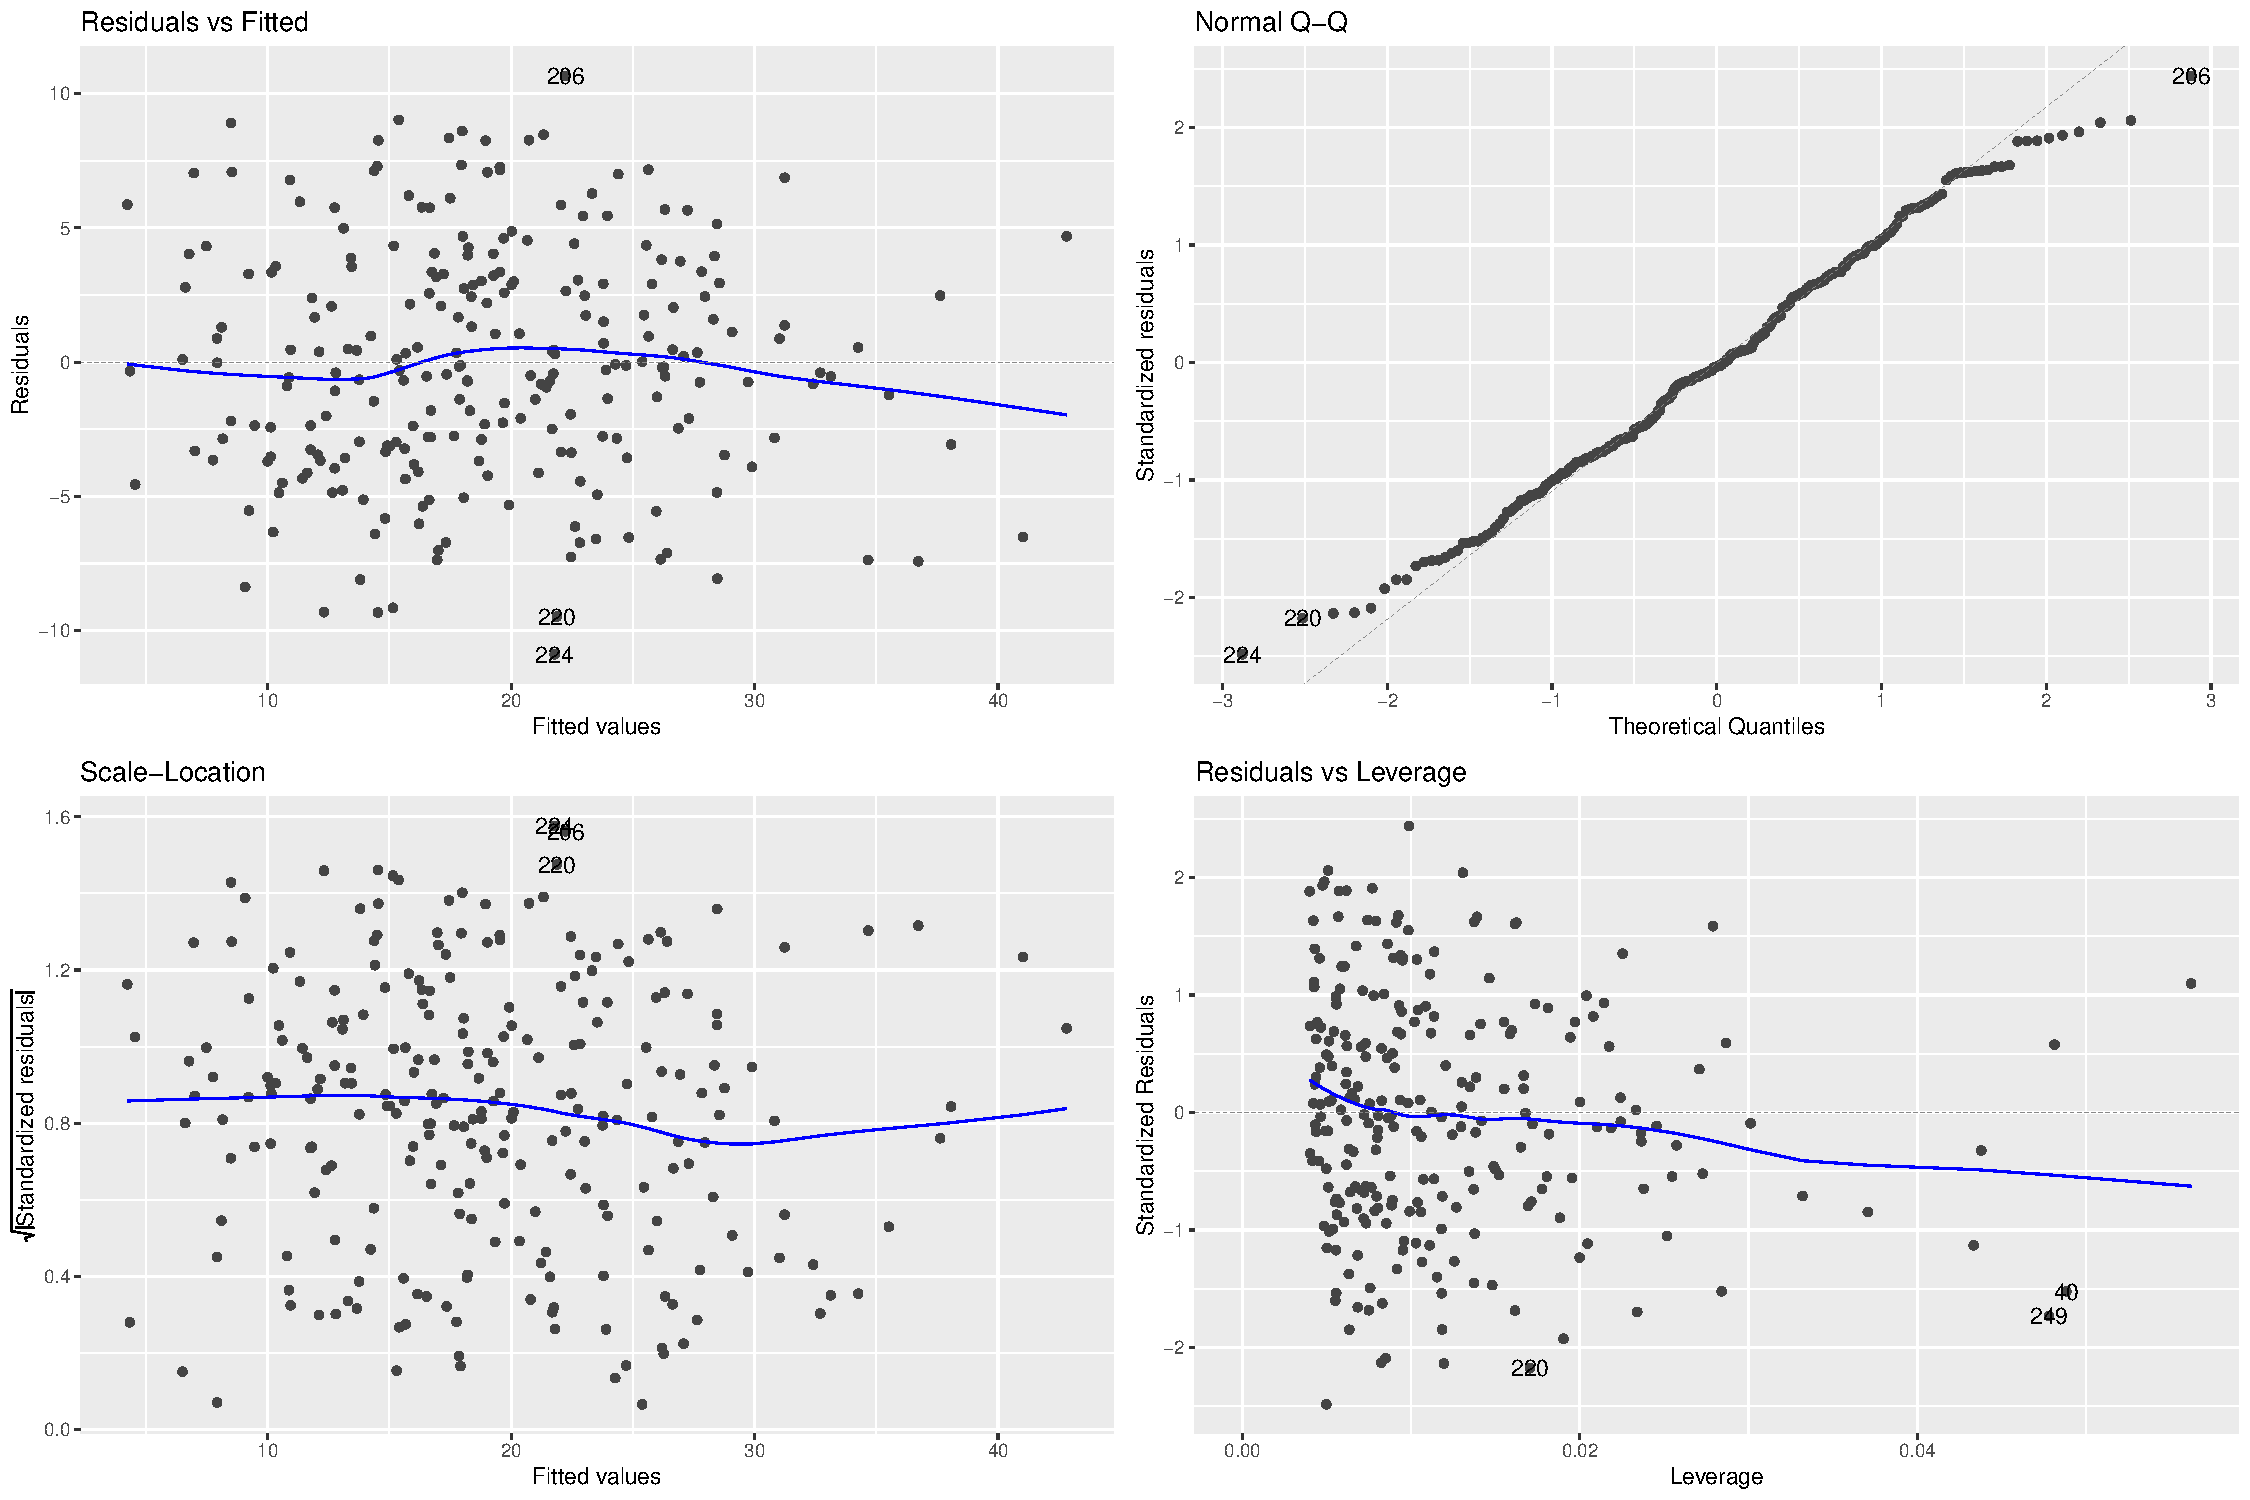
\includegraphics[width=0.95\linewidth]{Images/FIGURES/2var_linear_regression}
	\caption{2-variable linear regression results diagram.}
	\label{fig:2var_linear_regression}
\end{figure}

\subsection{Multiple Linear Regression}

\subsubsection{All Variables Included}

Now we will consider the model with almost all available variables and once again attempt to explain the fat percentage given by Siri's equation. The model is as follows, $\forall i \in \{1,2, \dots, 251\}$:\footnote{In contrast with the previous section, we also exclude the intercept from the model from by reason of common sense: with decreasing values of explanatory variables the fat percentage also decreases.}

\begin{equation}
	Y_{i} = \sum_{j = 1}^{15}\beta_{j} X_{i,\,j} + e_{i}
\end{equation}

\noindent
\medskip

or $Y = X \beta + e$ in a matrix form. Estimated values are displayed in the Tab.~\ref{tab:multivar_regression}. The R-squared statistic is quite high for the observed model and is equal to $0.995$ which means, that almost all of the response data variability is explained. Nonetheless, a lot of confidence intervals for estimated parameters contain zero. Moreover, residuals are not normally distributed (see Fig.~\ref{fig:multivar_linear_regression_all}), as the null hypothesis in the Lilliefors test is rejected due to the p-value equal to $5.101 \cdot 10^{-7}$. Thus, linear regression cannot be used for this set of explanatory variables.

\begin{table}[H]
	\centering
	\begin{tabular}{|c||c||c|c|}
		\hline 
		Parameter &  Estimated Value & \multicolumn{2}{c|}{Confidence Interval, $95\%$}  \\ 
		\hline \hline 
		Age, $\beta_{1}$ & 0.01 & -0.01 &  0.04 \\ 
		\hline 
		Total Weight, $\beta_{2}$ & 0.89 & 0.84 &  0.95 \\ 
		\hline 
		Height, $\beta_{3}$ & 0.01 & -0.01 & 0.04 \\ 
		Adiposity, $\beta_{4}$ & -0.27 & -0.47 & -0.06  \\
		\hline 
		Fat-free weight, $\beta_{5}$ & -1.23 & -1.29 & -1.18  \\
		\hline
		Neck CC, $\beta_{6}$ & 0.05 & -0.1 & 0.2  \\
		\hline
		Chest CC, $\beta_{7}$ & 0.02 & -0.04 & 0.09  \\
		\hline
		Abdomen CC, $\beta_{8}$ & 0.1 & 0.03 & 0.18  \\
		\hline
		Hip CC, $\beta_{9}$ & -0.01 & -0.09 & 0.07  \\
		\hline
		Thigh CC, $\beta_{10}$ & 0.13 & 0.04 & 0.23  \\
		\hline
		Knee CC, $\beta_{11}$ & 0.05 & -0.1 & 0.21  \\
		\hline
		Ankle CC, $\beta_{12}$ & 0.12 & -0.02 & 0.26  \\
		\hline
		Biceps CC, $\beta_{13}$ & 0.12 & 0.01 & 0.23  \\
		\hline
		Forearm CC, $\beta_{14}$ & 0.08 & -0.05 & 0.22  \\
		\hline
		Wrist CC, $\beta_{15}$ & -0.07 & -0.42 & 0.28  \\
		\hline
	\end{tabular} 
	\caption{Estimated values for the multivariate linear regression with all parameters included.}
	\label{tab:multivar_regression}
\end{table}

\begin{figure}[H]
	\centering
	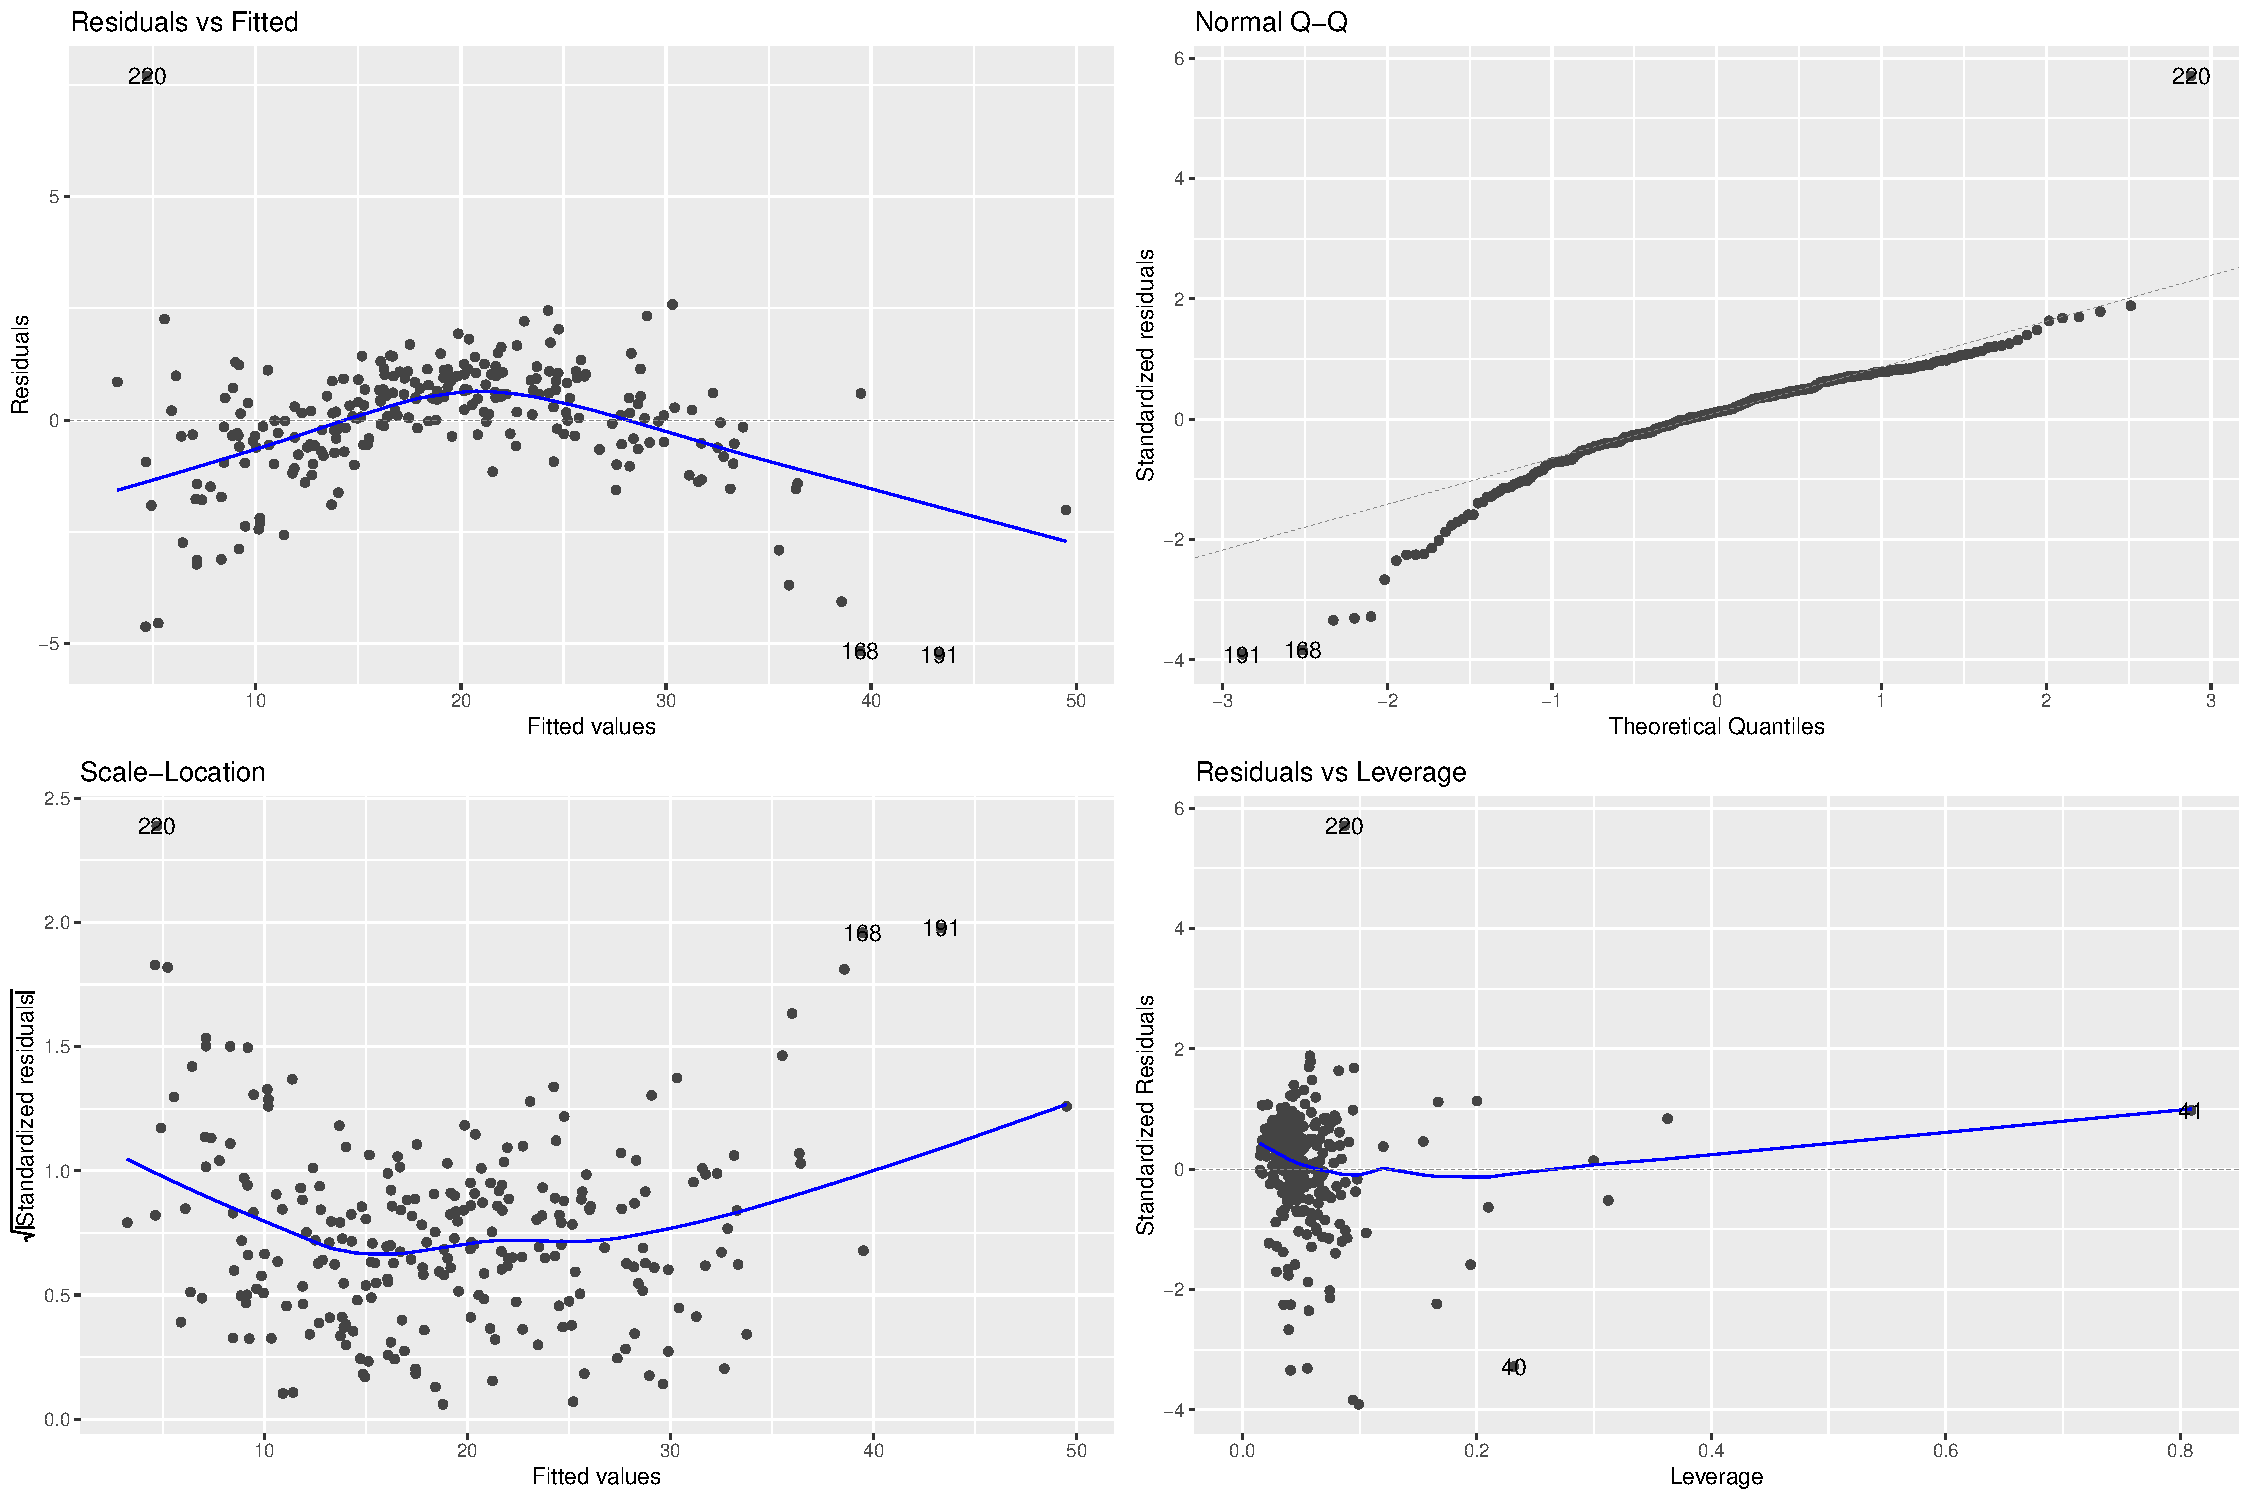
\includegraphics[width=0.95\linewidth]{Images/FIGURES/multivar_linear_regression_all}
	\caption{Multiple linear regression results diagram for the model with all variables included.}
	\label{fig:multivar_linear_regression_all}
\end{figure}

\subsubsection{The Final Model}

To make regression more sufficient, we exclude the total weight from the model due to its strong correlation ($0.76$) with the fat-free weight and run a stepwise algorithm to choose the the model by the Akaike Information Criterion. After excluding variables with low significance, we construct the final linear model using only  $8$ columns of the provided dataset: age, adiposity, fat-free weight, abdomen CC, hip CC, knee CC, biceps CC and wrist CC. Estimates of parameters are available in the Tab.~\ref{tab:multivar_regression_final}. Fortunately, the R-squared statistic has remained high: $R^{2} = 0.9766$., thus, almost all of the variability of the response variable is accounted for by our model.

\begin{table}[H]
	\centering
	\begin{tabular}{|c||c||c|c|}
		\hline 
		Parameter &  Estimated Value & \multicolumn{2}{c|}{Confidence Interval, $95\%$}  \\ 
		\hline \hline 
		Age, $\beta_{1}$ & -0.05 & -0.09 &  -0.01 \\ 
		\hline 
		Adiposity, $\beta_{2}$ & 0.52 & 0.19 & 0.85  \\
		\hline 
		Fat-free weight, $\beta_{3}$ & -0.57 & -0.65 & -0.49  \\
		\hline
		Abdomen CC, $\beta_{4}$ & 0.72 & 0.6 & 0.84  \\
		\hline
		Hip CC, $\beta_{5}$ & -0.19 & -0.34 & -0.03  \\
		\hline
		Knee CC, $\beta_{6}$ & 0.34 & 0.02 & 0.66  \\
		\hline
		Biceps CC, $\beta_{7}$ & 0.38 & 0.16 & 0.61  \\
		\hline
		Wrist CC, $\beta_{8}$ & -1.54 & -2.13 & -0.95  \\
		\hline
	\end{tabular} 
	\caption{Estimated values for the multivariate linear regression with all parameters included.}
	\label{tab:multivar_regression_final}
\end{table}

\medskip

As can be seen, confidence intervals no longer contain zero values. As for residuals (see Fig.~\ref{fig:multivar_linear_regression_final}), their normality is evident. Moreover, the Lilliefors test with statistical significance set to $5\%$ has resulted in our inability to reject the null hypothesis, as the p-value is equal to $0.4$. Hence, residuals distribution may be considered normal and we are eligible to use this model to perform multivariate linear regression.

\begin{figure}[H]
	\centering
	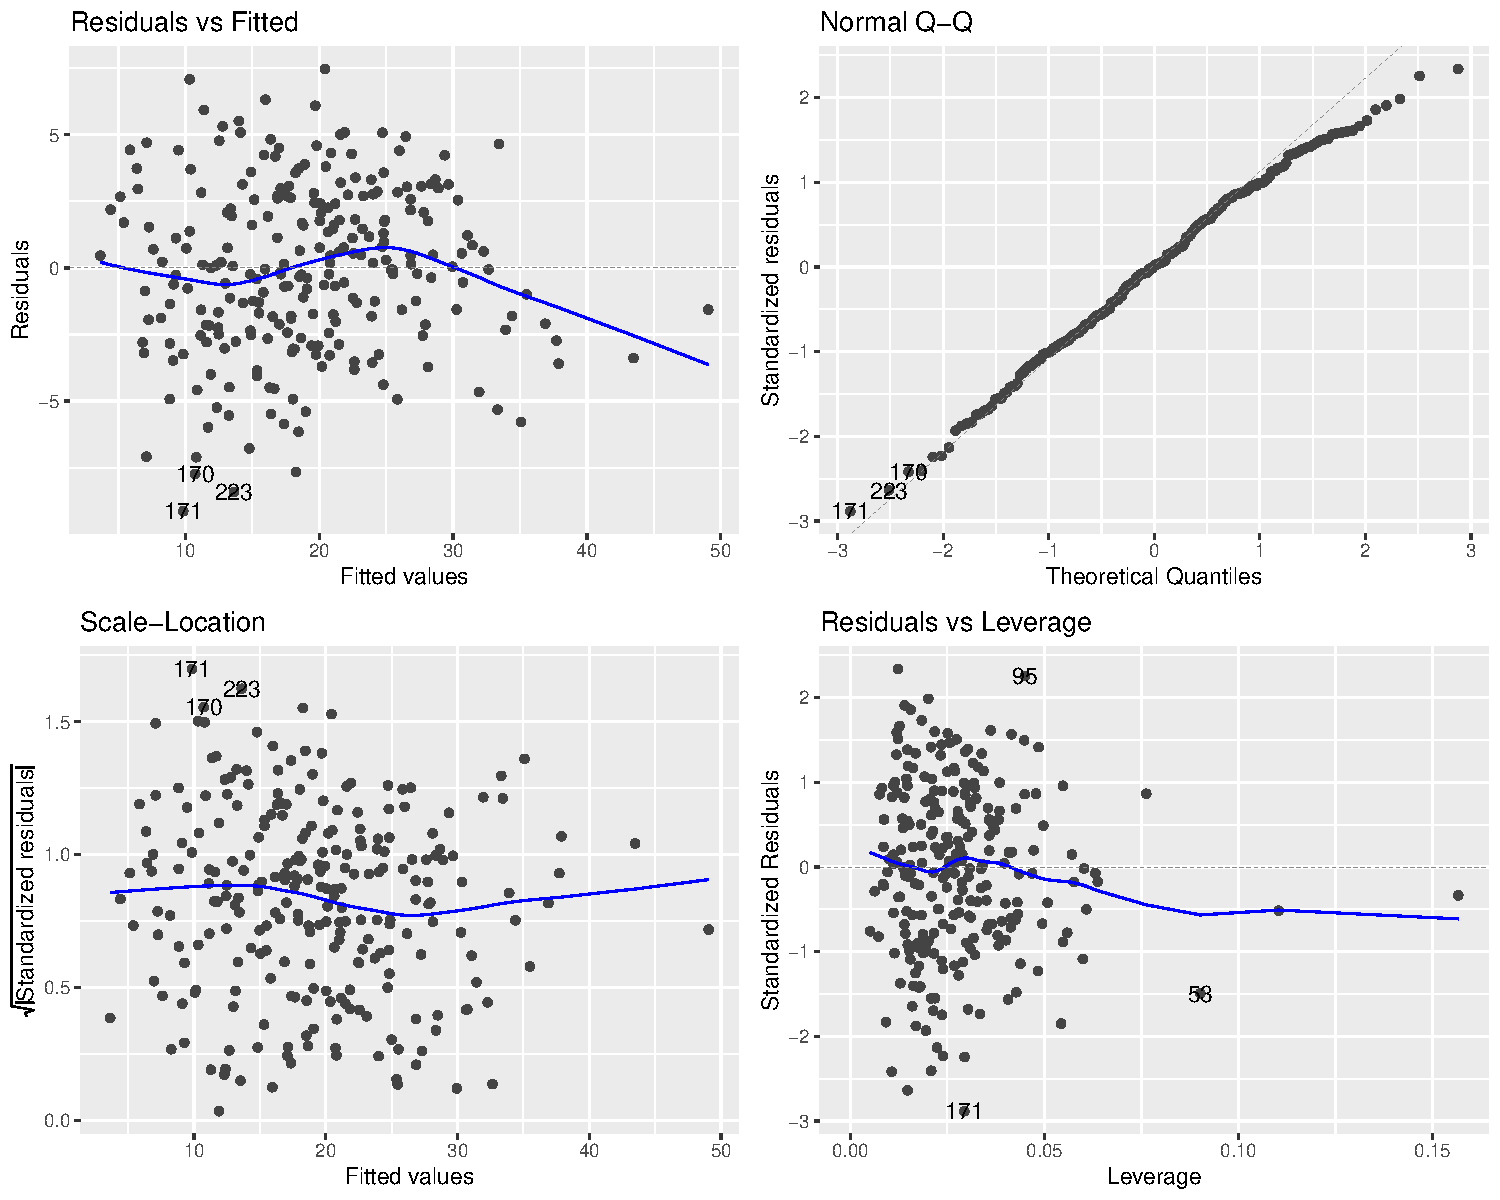
\includegraphics[width=0.95\linewidth]{Images/FIGURES/multivar_linear_regression_final}
	\caption{Multiple linear regression results diagram for the final model.}
	\label{fig:multivar_linear_regression_final}
\end{figure}

\newpage

%\newpage{}
%
%\bibliography{bib/Benes2017,bib/MMC}
%
%%\bibliographystyle{plain}
%\bibliographystyle{alpha}

\end{document}
